%CLASSE DOCUMENTO - LINGUA E DIMENSIONE FONT
\documentclass[a4paper, 
				11pt,
				stile=classica,
				tipotesi=triennale]{toptesi}

%%%%%%%%%%%%%%%%%%%%%%%%%%%%%%%%%%%%%%%%%%%%%%%%%%%%%%%%%%%%%%%

% INCLUSIONE PACCHETTI
\usepackage[utf8]{inputenc} %utf8
\usepackage[italian]{babel}
\usepackage[T1]{fontenc}
\usepackage{blindtext}
\usepackage{graphicx,wrapfig}
\usepackage{booktabs}
\usepackage{lmodern}
\usepackage{varioref}
\usepackage{url}
\usepackage{array}
\usepackage{paralist}{\obeyspaces\global\let =\space}
\usepackage{verbatim} 
\usepackage{subfig}
\usepackage{tabularx}
\usepackage{amsmath}
\usepackage{amsfonts}
\usepackage{float}
\usepackage{amssymb}
\usepackage{multicol}
\usepackage{multirow}
\usepackage{listings}
\usepackage[pass]{geometry}
\usepackage[figuresright]{rotating}
\usepackage{algorithm}
\usepackage{algorithmic}
\usepackage{amsmath}
\usepackage[babel]{csquotes}
\usepackage{hyperref}
\usepackage[backend=bibtex]{biblatex}

%%%%%%%%%%%%%%%%%%%%%%%%%%%%%%%%%%%%%%%%%%%%%%%%%%%%%%%%%%%%%%%



% CONFIGURAZIONE LINK E RIFERIMENTI
\hypersetup{%
    pdfpagemode={UseOutlines},
    bookmarksopen,
    pdfstartview={FitH},
    colorlinks,
    linkcolor={black}, %COLORE DEI RIFERIMENTI AL TESTO
    citecolor={blue}, %COLORE DEI RIFERIMENTI ALLE CITAZIONI
    urlcolor={blue} %COLORI DEGLI URL
}

%%%%%%%%%%%%%%%%%%%%%%%%%%%%%%%%%%%%%%%%%%%%%%%%%%%%%%%%%%%%%%%

% CONFIGURAZIONE LISTATI/CODICE - CANCELLARE SE NON NECESSARIO
% PYTHON - BIANCO E NERO
\lstset{%
	captionpos=b,
	language=Java,
	basicstyle =\small\ttfamily,
	keywordstyle=\color{black}\bfseries,
	breaklines=true,
	breakatwhitespace=true,
	frame=lines,
	numbers=left,
	numberstyle=\footnotesize,
}

%%%%%%%%%%%%%%%%%%%%%%%%%%%%%%%%%%%%%%%%%%%%%%%%%%%%%%%%%%%%%%%

% FRENCHSPACING VA _SEMPRE_ ABILITATO PER DOCUMENTI IN ITALIANO
\frenchspacing

%%%%%%%%%%%%%%%%%%%%%%%%%%%%%%%%%%%%%%%%%%%%%%%%%%%%%%%%%%%%%%%

%Rinominato il menu dei listati
\renewcommand\lstlistingname{Listato}
\renewcommand\lstlistlistingname{Elenco dei Listati}


\setcounter{tocdepth}{3}
\setcounter{secnumdepth}{4}
%%%%%%%%%%%%%%%%%%%%%%%%%%%%%%%%%%%%%%%%%%%%%%%%%%%%%%%%%%%%%%%

%DEFINIZIONE SEZIONI IN NUMERAZIONE ROMANA
%ELENCO DEI LISTATI/CODICI
\makeatletter
\newcommand\listofcodes{%
 \iffrontmatter\else\frontmattertrue\fi
 \if@openright\cleardoublepage\else\clearpage\fi
 % change the meaning of \chapter in a group
 \begingroup\def\chapter##1{\@schapter}
 \phantomsection % for the hyperlink
 \lstlistoflistings 
 \endgroup
} 
\makeatother

%%%%%%%%%%%%%%%%%%%%%%%%%%%%%%%%%%%%%%%%%%%%%%%%%%%%%%%%%%%%%%%

% INFORMAZIONI PDF - PERSONALIZZARE
\pdfinfo{%
  /Title    (PROGETTAZIONE E SVILUPPO DI UN SISTEMA DISTRIBUITO PER L'ANALISI DELLE TRANSAZIONI BITCOIN)
  /Author   (Antonio Riccardi)
  /Keywords (bitcoin;blockchain;spark;neo4j;nodejs)
}


% LISTA DEI CAPITOLI DA INCLUDERE - PERSONALIZZARE
\includeonly{%
intro,%
overview,%
implementazione,%
conclusioni,%
app_a,%
}

% FILE DI BIBLIOGRAFIA
\bibliography{bibliography} 




%%%%%%%%%%%%%%%%%%%%%%%%%%%%%%%%%%%%%%%%%%%%%%%%%%%%%%%%%%%%%%%

% INIZIO DOCUMENTO
\begin{document}


\begin{ThesisTitlePage}
    % FRONTESPIZIO - PERSONALIZZARE
	% ELIMINATE LE VOCI CHE NON VI SERVONO

	% UNIVERSITA - NOME
	\ateneo{Universit\`a degli Studi di Napoli "Parthenope"}

	% FACOLTA - DICITURA - CANCELLARE O DECOMMENTARE
	%\FacoltaDi{Faculty of}
	% FACOLTA - NOME
	\nomeateneo{Dipartimento di Scienze e Tecnologie}

	% CORSO DI LAUREA - DICITURA (MANTENERE LO SPAZIO) - CANCELLARE O DECOMMENTARE
	%\CorsoDiLaureaIn{Master of Science in }
	% CORSO DI LAUREA - NOME
	\corsodistudi{Corso di Laurea in Informatica}


	% TIPOLOGIA TESI
	\NomeElaborato{Tesi di Laurea Triennale}

	% TITOLO
	\titolo{PROGETTAZIONE E SVILUPPO DI UN SISTEMA DISTRIBUITO PER L'ANALISI DELLE TRANSAZIONI BITCOIN}

	% RELATORE/I - DICITURA - CANCELLARE SE UN SOLO RELATORE
	%\AdvisorName{Relatori}
	% RELATORE - PROF. NOME E COGNOME
	\relatore{prof. Alessio Ferone}


	% CANDIDATO - NOME E COGNOME
	\candidato{Antonio Riccardi \\mat. 0124000411}

	% LOGO UNIVERSITA
	\logosede{images/logo}

	% DATA - MESE ANNO
	\sedutadilaurea{Anno accademico 2018 - 2019}
    
\end{ThesisTitlePage}

%INTERLINEA - DEFAULT 1 - NON ESAGERATE, NON SUPERATE MAI 1.3 ;)
\interlinea{1.0}

%%%%%%%%%%%%%%%%%%%%%%%%%%%%%%%%%%%%%%%%%%%%%%%%%%%%%%%%%%%%%%%

\frontmatter

% DEDICA - PERSONALIZZARE
% VSPACE - PROPORZIONE USATA PER CENTRATURA VERTICALE DEL TESTO
% FLUSHRIGHT - ALLINEAMENTO ORIZZONTALE A DESTRA
\vspace*{\stretch{1}}
\begin{flushright}
\noindent
	Ai miei genitori.
\end{flushright}
\vspace*{\stretch{6}}
\cleardoublepage


%%%%%%%%%%%%%%%%%%%%%%%%%%%%%%%%%%%%%%%%%%%%%%%%%%%%%%%%%%%%%%%

% RINGRAZIAMENTI - PERSONALIZZARE
\ringraziamenti
TODO \\Grazie a soreta.

%%%%%%%%%%%%%%%%%%%%%%%%%%%%%%%%%%%%%%%%%%%%%%%%%%%%%%%%%%%%%%%

% ABSTRACT - PERSONALIZZARE
\sommario
La seguente tesi ha come obiettivo la realizzazione di un'applicazione distribuita in grado di fare analisi di transazioni provenienti dalla blockchain di Bitcoin.\\Il nocciolo della questione affrontata è quello di studiare la struttura di ogni singola piattaforma distribuita e di implementare componenti in grado di ricavare informazioni utili per l'analisi delle transazioni. In particolare, ci si soffermerà sulle principali tecnologie informatiche che permettono di costruire sistemi distribuiti, come Spark ed Hadoop, e sulle strutture dati che facilitano l'immagazzinamento delle informazioni come Neo4j.
\\Nella prima parte della tesi si procede con l'introduzione alla tecnologia alla base della moneta virtuale Bitcoin, facendo luce su cos’\'e la Blockchain e quali vantaggi/svantaggi presenta rispetto ad altri sistemi che gestiscono transazioni monetarie. A seguire, sono presi in esame le principali soluzioni di analisi di transazioni gi\'a esistenti. 
\\Il secondo capitolo dell'elaborato mostra una panoramica del disegno dell’architettura del sistema realizzato, mettendo in luce i principali componenti del sistema. A tal fine è presente un'ampia e dettagliata descrizione di ogni singolo componente del sistema specificando i vantaggi ottenuti dal proprio utilizzo.
\\Il terzo capitolo descrive come è stata fatta l'implementazione del sistema, mostrando porzioni di codice e screen dell'applicazione che ci aiutano nella comprensione di come funziona il sistema.
\\Infine nell'ultimo capitolo vengono trattate le considerazioni finali del lavoro svolto soffermandosi anche sui possibili sviluppi. 

%%%%%%%%%%%%%%%%%%%%%%%%%%%%%%%%%%%%%%%%%%%%%%%%%%%%%%%%%%%%%%%


% INDICI - ELIMINARE GLI INDICI NON NECESSARI

% INDICE GENERALE
\tableofcontents

% INDICE DELLE FIGURE
\listoffigures

% INDICE DELLE TABELLE
\listoftables

% INDICE DEI CODICI

\listofcodes
\addcontentsline{toc}{chapter}{Elenco dei Listati}
%%%%%%%%%%%%%%%%%%%%%%%%%%%%%%%%%%%%%%%%%%%%%%%%%%%%%%%%%%%%%%%

\mainmatter
\setcounter{secnumdepth}{4}

% INCLUSIONE FILE CAPITOLI - PERSONALIZZARE - TENERE COERENTE CON LISTA IN ALTO
\chapter{Bitcoin: Fonte di bigdata}
\label{chap:bitcoin fonte di bigdata}

Nel lontano 2009 uno pseudonimo Satoshi Nakamoto pubblicò il manifesto \textit{"Bitcoin: A Peer-to-Peer Electronic Cash System"}\cite{bitcoin:white-paper} sancendo la nascita di una nuova moneta digitale chiamata Bitcoin, che fa  del suo punto di forza la libertà e la sicurezza. Nel corso degli anni il valore della moneta è cresciuto sino a raggiungere picchi di 19290 dollari nel 17 Dicembre 2017 \cite{blockchain.com:valueOf}. Di pari passo, anche il numero di transazioni giornaliere sulla rete bitcoin ha raggiunto cifre esorbitanti riuscendo a validare 5 transazioni al secondo\cite{blockchain.com:transactions}, questa enorme mole di dati è possibile processarla solo con sistemi distribuiti che gestiscono i Big Data. Quest'ultimi rappresentano tutti quei dati che possono essere disponibili in enormi volumi, possono presentarsi con formati semistrutturati o addirittura destrutturati e possono essere prodotti con estrema velocità. Uno degli aspetti che caratterizzano i big data è la loro quantità. Questi dati infatti, sono generati dall'utente attraverso gli strumenti del Web 2.0, sistemi gestionali, oppure generati automaticamente da macchine (sensori, sistemi di calcolo) assumendo volumi rilevanti, non più gestibili con strumenti di database tradizionali. Non a caso l'elaborato di tesi, utilizza un sistema distribuito creato ad hoc per i big data per gestire l'enorme volume di transazioni che circolano nella rete Bitcoin.
\\Bitcoin, oltre all'impatto economico, ha avuto un importante ruolo nel campo della ricerca, donandoci un sistema che gestisce le transazioni tra due parti in un network peer-to-peer, diversamente dai sistemi tradizionali, denominato Blockchain.

\section{Blockchain}
\label{sec:blockchain}

La blockchain come dice il nome è una catena di blocchi che implementano un database  aperto e distribuito, atto a memorizzare le transazioni tra due parti in modo sicuro, verificabile e permanente. In altre parole, la blockchain rappresenta il libro contabile (o libro mastro), ossia il registro sul quale sono riportati tutti gli scambi tra le parti. Questo libro mastro è distribuito (Distributed Ledger) replicato e sincronizzato tra tutti i membri di una rete. In questo database vengono registrate le transazioni (come lo scambio di beni o informazioni) tra i partecipanti alla rete.
\\I dati non sono memorizzati su un solo computer ma su più macchine collegate tra loro attraverso una rete peer-to-peer [\ref{fig:blockchainNetwork}] sottoforma di blocchi.
\\Ciascun nodo è autorizzato ad aggiornare e gestire il libro contabile distribuito in modo indipendente, ma sotto il controllo consensuale degli altri nodi. Infatti, gli aggiornamenti non sono più gestiti, come accadeva tradizionalmente, sotto il controllo rigoroso di un’autorità centrale, ma sono invece creati e caricati da ciascun nodo in modo appunto indipendente. In questo modo ogni partecipante è in grado di processare e controllare ogni transazione ma, nello stesso tempo ogni singola transazione, essendo gestita in autonomia, deve essere verificata, crittografata e approvata dalla maggioranza dei partecipanti alla rete. 

\begin{figure}[H]
	\centering
	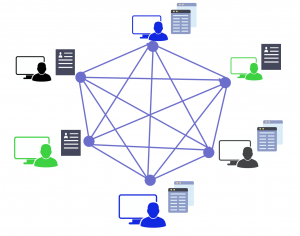
\includegraphics[width=0.5\textwidth]{images/blockchainNetwork.png}
	\caption{Rete distribuita di nodi paritari.}
	\label{fig:blockchainNetwork}
\end{figure}

Ogni blocco contenuto nella blochchain archivia un insieme di transazioni validate correlate da un Marcatore Temporale (Timestamp) ed un hash (una stringa alfanumerica) che identifica il blocco in modo univoco e che permette il collegamento con il blocco precedente[\ref{fig:blockChain}].

\begin{figure}[H]
	\centering
	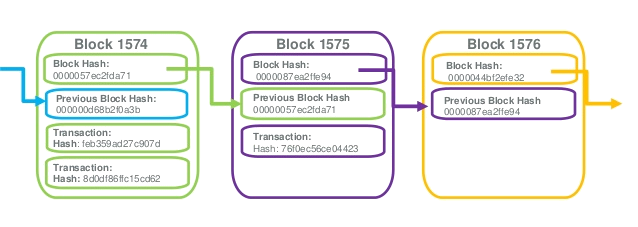
\includegraphics[width=\textwidth]{images/blockChain.png}
	\caption{Catena di blocchi nella blockchain.}
	\label{fig:blockChain}
\end{figure}

Perché un nuovo blocco di transazioni sia aggiunto alla Blockchain è necessario appunto che sia controllato, validato e crittografato. Solo con questo passaggio può poi diventare attivo ed essere aggiunto alla Blockchain. Per effettuare questo passaggio è necessario che ogni volta che viene composto un blocco venga risolto un complesso problema matematico che richiede un cospicuo impegno anche in termini di potenza e di capacità elaborativa. Questa operazione viene definita come “Mining” ed è svolta dai “Miner”. La risoluzione del problema è un processo irreversibile per cui il blocco valido aggiunto alla catena diviene immutabile.
\\In conclusione, questa tecnologia può essere utilizzata in tutti gli ambiti in cui è necessaria una relazione tra più persone o gruppi. Ad esempio può garantire il corretto scambio di titoli e azioni o sostituire un atto notarile, perché ogni transazione viene sorvegliata da una rete di nodi che ne garantiscono la correttezza senza l’ausilio di intermediari.
\\Bitcoin sfrutta questa tecnologia per gestire le transazioni finanziarie in modo sicuro e del tutto autonomo.
\section{Bitcoin}
\label{sec:bitcoin}
Bitcoin (codice: BTC o XBT) è una criptovaluta e un sistema di pagamento mondiale creato nel 2009 da un anonimo inventore, noto con lo pseudonimo di Satoshi Nakamoto, che sviluppò un'idea da lui stesso presentata su Internet a fine 2008. Per convenzione se il termine Bitcoin è utilizzato con l'iniziale maiuscola si riferisce alla tecnologia e alla rete, mentre se minuscola (bitcoin) si riferisce alla valuta in sé.\cite{bitcoin:ECDSA}
\\Il progetto Bitcoin è nato con l'intento di risolvere i problemi di fiducia, trasparenza e responsabilità tra due parti nello scambio di denaro per beni e servizi su Internet, senza l'utilizzo di intermediari. Bitcoin, infatti, rappresenta la prima rete di pagamento che utilizza una tecnologia distribuita peer-to-peer per operare senza un'autorità centrale: la gestione delle transazioni e l'emissione di denaro sono effettuati collettivamente dalla rete.
\\La rete Bitcoin utilizzando la tecnologia blockchain, è una catena di blocchi concatenati tra di loro, infatti ogni blocco contiene il riferimento al hash del blocco precedente. Questo sistema è immutabile perchè se si volesse modificare un blocco si dovrebbero modificare tutti i blocchi successivi ad esso, per fare ciò si dovrebbe creare una catena di blocchi che è più lunga di quella esistente. Ovviamente, la distribuzione e la natura delle tempistiche del processo rendono praticamente impossibile che ciò accada.
\\Inotre, utilizzando un sistema distribuito, permette di tenere traccia di tutti i trasferimenti in modo da evitare il problema del double spending (spendere due volte). Tutti gli utenti sono a conoscenza di ciò che accade e pertanto non c’è bisogno di una autorità centrale che gestisca le transazioni.
\\In aggiunta, Bitcoin consente il possesso e il trasferimento anonimo delle monete, ed infatti i dati necessari per usufruire dei propri bitcoin sono salvati in uno o più personal computer sotto forma di digital wallet (portafoglio). I bitcoin sono trasferiti tramite Internet a chiunque disponga di un indirizzo bitcoin. La struttura peer-to-peer della rete e l'assenza di un ente centrale rende impossibile a qualsiasi autorità il blocco dei trasferimenti, il sequestro dei bitcoin senza il possesso delle relative chiavi o la svalutazione dovuta all'immissione di nuova moneta. Per questo motivo i bitcoin sono la moneta più utilizzata nel Deep Web.
\\
\\Ricapitolando, le principali caratteristiche su cui si basa questo sistema di enorme successo sono le seguenti:
\begin{itemize}
\item \textbf{Nessuna autorità centrale}: non dipende da nessuna terza parte privata o ente governativo, e, pertanto, il valore dei BTC è liberamente contrattato sul mercato. Si tratta quindi di un sistema decentralizzato;
\item \textbf{Irreversibile e non falsificabile}: una volta che una transazione è stata effettuata ed è inclusa nella blockchain, non può più essere annullata, nemmeno dal mittente;
\item \textbf{Anonimo}: chiunque può scaricare il software ed iniziare ad effettuare transazioni senza registrarsi, comunicare dati personali e senza svelare la propria identità.
\item \textbf{Sistema distribuito su rete Peer-to-peer (rete paritaria o paritetica)}: qualsiasi nodo è in grado di avviare e completare una transazione in modo autonomo.
\item \textbf{Inflazione determinata a priori}: L’emissione di nuovi BTC è determinata dall’algoritmo stesso del programma, e non può essere modificata.
\end{itemize}
Per capire meglio questi punti, verrà illustrata in modo dettagliato una transazione tra due utenti Alice e Bob che vogliono scambiarsi bitcoin.

\begin{figure}[H]
	\centering
	
\includegraphics[width=0.3\textwidth]{images/bitcoinLogo.png}
	\caption{Logo Bitcoin.}
	\label{fig:bitcoinLogo}
\end{figure}

\subsection{Come avviene una transazione}
\label{sec:come avviene una transazione}
Un esempio pratico di scambio di moneta aiuterà nel capire come funziona il sistema. I nostri attori saranno Alice (pagante) e Bob (ricevente).
\\
\\I passi da eseguire sono:
\begin{enumerate}\itemsep2pt

\item Bob comanda alla sua applicazione (wallet) su PC o smartphone di creare un indirizzo. Il software restituisce una sequenza alfanumerica da 26 a 35 caratteri. Questo è un esempio: 12gXGyXWkvyDAjVKZHyGGstVYyXJ6ZjgqV

\item Bob copia l'indirizzo e lo mostra al mittente tramite qualunque mezzo: via mail, messaggio, QR code, pubblicato su un sito internet, scritto su carta, dettato al telefono etc.

\item Alice inserisce nel suo software l'indirizzo di Bob e la quantità di Bitcoin da inviare, inoltre specifica l'ammontare della commissione da pagare al minatore (detto "miner") per convalidare la transazione. Ad oggi i più comuni software stabiliscono automaticamente una commisione fissa a 0,00001 bitcoin.

\item Bob ritrova sul suo software la transazione avvenuta, ma prima di considerare il pagamento effettuato attende che la transazione sia inserita nella blockchain.

\item In un massimo di 10 minuti circa la transazione viene inserita in un blocco della blockchain da parte del miner, che ha convenienza a inserirla perché in questo modo ottiene la commissione pagata da Alice.

\item Bob può sentirsi sicuro che la transazione è confermata con l’aumentare di blocchi che vengono aggiunti alla blockchain conseguentemente a quello che contiene la transazione. 

\item Bob avrà nel proprio portafoglio i bitcoin inviati da Alice per spenderli in una nuova transazione.
\end{enumerate}

\begin{figure}[H]
	\centering
	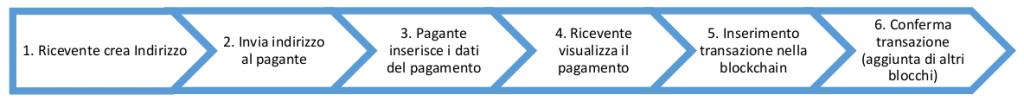
\includegraphics[width=\textwidth]{images/transazioneBitcoin.png}
	\caption{Come avviene una transazione Bitcoin.}
	\label{fig:bitcoinTransaction}
\end{figure}

\subsection{Come avviene una transazione dal punto di vista tecnico}
\label{sec:come avviene una transazione dal punto di vista tecnico}
La stessa transazione viene affrontata con un occhio più tecnico, soffermando l'attenzione sulla parte di creazione delle chiavi e della conferma ed aggiunta del blocco.
\\
\\I passi da eseguire sono:
\begin{enumerate}\itemsep2pt
\item Tramite il software che si occupa del wallet, Bob genera in modo del tutto casuale una chiave privata, che viene salvata sul suo computer.
\item La chiave privata viene convertita in una chiave pubblica tramite un procedimento matematico. Comunemente è il software di Bob a generare automaticamente la chiavi quando Bob chiede all'applicazione di creare un indirizzo da comunicare al mittente. In realtà Bob potrebbe utilizzare una chiave privata facilmente ricordabile, come “sum qui sum”, e ricavare Public key e indirizzo da questa. Il procedimento matematico si basa su un algoritmo chiamato “Elliptic Curve Digital Signature Algorithm”\cite{bitcoin:ECDSA} che utilizza la curva ellittica.
\\È teoricamente possibile ma statisticamente impraticabile scoprire la chiave privata partendo da quella pubblica: poiché il procedimento matematico applicato è unidirezionale, il processo inverso per indovinare la chiave privata richiederebbe una quantità di tentativi e una potenza di calcolo talmente enorme da essere al di là di ogni possibilità
\item La chiave pubblica viene a sua volta crittografata e accorciata tramite un hash. Possiamo chiamare la nuova chiave pubblica Public Key Hash. La chiave pubblica originaria invece è detta Full Public Key.
\item L'hash della chiave pubblica viene convertito in una riga di massimo 35 caratteri (per comodità pratica), che costituisce l'indirizzo del portafoglio di Bob. Per esempio: 12gXGyXWkvyDAjVKZHyGGstVYyXJ6ZjgqV.
\item Bob spedisce l'indirizzo ad Alice.
\begin{figure}[H]
	\centering
	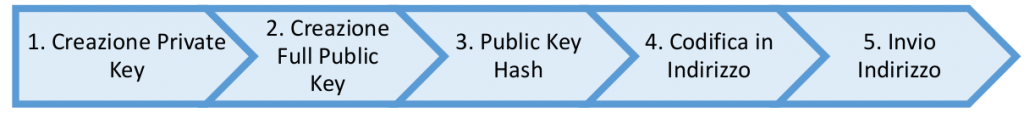
\includegraphics[width=\textwidth]{images/passiDiBob.png}
	\caption{Azioni del ricevente.}
	\label{fig:bobSteps}
\end{figure}
\item Il software di Alice decodifica immediatamente l'indirizzo in una normale Public Key Hash
\item \label{aliceCreaTransazione} Alice crea la transazione. Si può pensare la transazione come un codice che contiene diverse informazioni, ciascuna rappresentabile come una stringa composta da molti caratteri:
\begin{itemize}
\item l’input: uno o più output di una transazione precedente fatta nei confronti di Alice, da cui ella attinge i bitcoin che «spedisce» nel nuovo output
\item l'output: la quantità di bitcoin spediti. Possono esserci più output per ogni transazione, ciascuno identificato con un ID specifico
\item l'istruzione per la firma (la "signature script"): ovvero le istruzioni che Bob dovrà fornire per convalidare la transazione, dimostrando di essere il possessore del nuovo output. È proprio per la creazione dello script che il software di Alice ha bisogno del Public Key Hash fornito da Bob. Le informazioni necessarie per validare la firma sono due, entrambe già in possesso di Bob: la full Public Key e la Private Key, che dovranno combaciare col Public Key Hash specificato da Alice nello script.
\end{itemize}
Queste informazioni vengono processate insieme nella creazione di un unico hash chiamato txid (transaction identifier)
\begin{figure}[H]
	\centering
	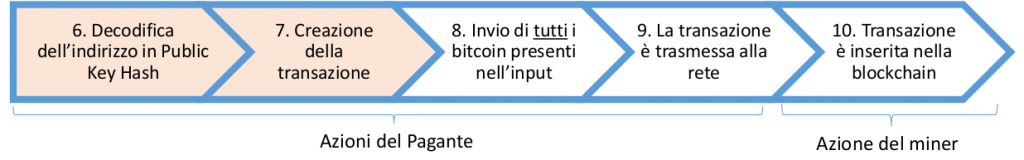
\includegraphics[width=\textwidth]{images/passiAlice1.png}
	\caption{Prima parte. Azioni del pagante.}
	\label{fig:aliceSteps1}
\end{figure}
\item Tutti i bitcoin che Alice ha a disposizione su un particolare input vengono "spediti" nella transazione. Infatti nella transazione è coinvolta sempre l'intera quantità di bitcoin presenti nell’input anche se Bob ne ha richiesti molti meno. Se Alice dispone di un input di 100 bitcoin e ne trasferisce 20 a Bob, l’input è sempre trasferito nella sua interezza di 100 bitcoin. In questo caso avrà due output diversi, uno di 80 bitcoin (al lordo della commissione per il miner) che tornano al portafoglio di Alice (il change output), l'altro di 20 bitcoin che vanno all'indirizzo di Bob. L’unico caso di transazione che abbia un solo input e un solo output è quello in cui l’input corrisponde esattamente all’ammontare richiesto da chi riceve i bitcoin. Spesso le transazioni hanno più output, e quindi i bitcoin trasferiti vanno ad indirizzi con diverse chiavi pubbliche e private.
\item Alice trasmette via internet al software di tutti gli altri nodi tutte le informazioni relative alla transazione. I nodi sono rappresentati da tutti coloro che hanno il software Bitcoin Core sui propri pc/dispositivi o numerosi altri software che permettono di "collegarsi" al network Bitcoin.
\begin{figure}[H]
	\centering
	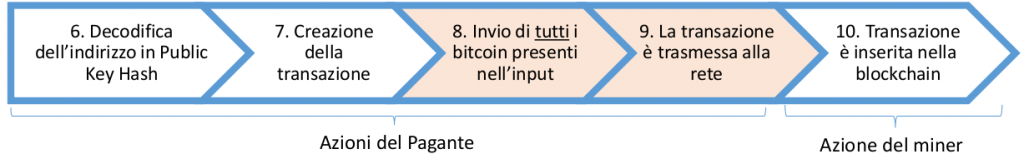
\includegraphics[width=\textwidth]{images/passiAlice2.png}
	\caption{Seconda parte. Azioni del pagante.}
	\label{fig:aliceSteps2}
\end{figure}

\item I minatori inseriscono le transazioni ancora non confermate nella blockchain.
\\Per inserire le transazioni all’interno della blockchain il miner deve creare un nuovo blocco, processo che richiede una quantità di calcolo molto elevata e dunque una spesa in energia elettrica e strumenti. Un miner ha interesse a inserire quante più transazioni nel blocco che vuole creare poiché guadagnerà tutte le commissioni pagate su ciascuna transazione. Se una transazione non include alcuna commissione, il miner non ha alcun interesse economico nell’inserirla nel blocco.

\begin{figure}[H]
	\centering
	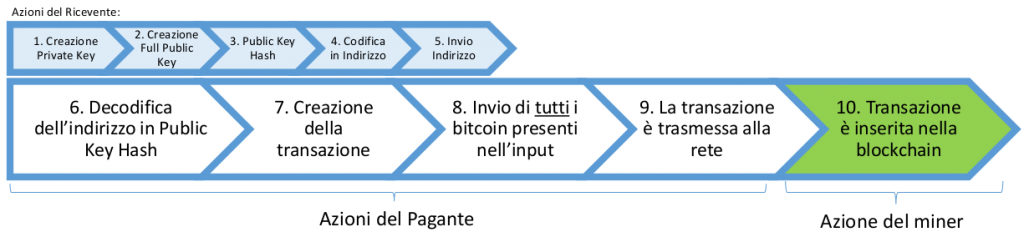
\includegraphics[width=\textwidth]{images/azioneMiner.png}
	\caption{Azione dei miner.}
	\label{fig:minerSteps}
\end{figure}

Per inserire le transazioni nel blocco, i minatori partono dagli id delle transazioni (txid), ciascuno dei quali rappresenta l’hash di tutte le informazioni inerenti una singola transazione (passo \ref{aliceCreaTransazione}).
\\I txid sono accoppiati due a due, creando un hash per ogni coppia di transazioni. Ogni hash viene poi accoppiato con un altro hash, creando un hash figlio dei due hash precedenti, e così via finché non si arriva a un unico hash. In caso di numeri dispari un hash viene processato con una sua copia identica. Questo procedimento può essere rappresentato come un albero, il cosiddetto Merkle tree [\ref{fig:merkelTree}],  dove le foglie sono le transazioni txid, i rami (biforcuti) gli hash intermedi e la radice l’hash finale, prodotto di tutti gli altri hash: la Merkle root. L’hash finale è come l’ultimo di una stirpe e porta con sé il “DNA” di tutti gli hash precedenti\cite{merkle-tree}.
\\Grazie alla struttura del Merkle tree, non è necessario conoscere tutte le transazioni incluse in un blocco per verificare che una singola transazione ne faccia parte, è invece sufficiente seguire un particolare ramo che collega una foglia (una transazione) alla merkle root.
\begin{figure}[H]
	\centering
	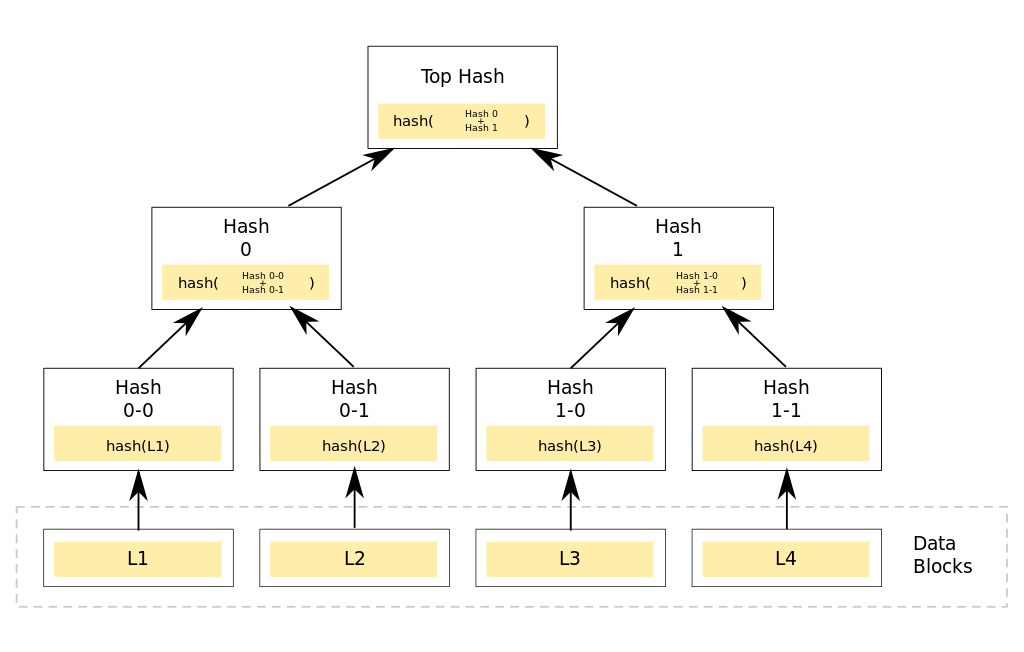
\includegraphics[width=\textwidth]{images/merkle_tree.png}
	\caption{Merkle tree.}
	\label{fig:merkelTree}
\end{figure}

\item Bob ora vuole spendere i suoi nuovi bitcoin in una nuova transazione, il destinatario è Charlie. Bob segue la stessa procedura che ha seguito Alice, creando una transazione specificando output, signature script (per cui gli serve il public key hash di Charlie), timestamp e versione del software.
\\Bob però deve dimostrare di essere il possessore dei bitcoin che invia a Charlie, ovvero i bitcoin presenti nell’input della transazione. Tale input è anche l’output della transazione fra Alice e Bob. Quest’ultimo per dimostrare di possedere l’ouput di quella transazione deve porre la sua firma (signature). Bob inserisce quindi la sua Full Public Key, verificando che corrisponde al Public Key Hash dato in precedenza ad Alice, e la sua Private Key, che rappresenta la conferma che Bob solo è la persona che ha originato inizialmente quella Public Key. Infatti seppur sia teoricamente possibile, è per motivi statistici «infattibile» scoprire la Private Key partendo dalla Public Key. Il procedimento di firma è del tutto automatizzato dal software Bitcoin\cite{transazioneBitcoin}.

\end{enumerate}
\section{Analisi dati su sitemi distribuiti}
\label{sec:analisi dati su sistemi distribuiti}
Il numero di utenti che ogni giorno spende bitcoin è in costante crescita. La tecnologia Bitcoin quindi è costretta a lavorare con volumi di dati sempre crescente. Per questo motivo, le applicazioni che fanno analisi devono adattarsi scegliendo sistemi consoni a queste moli di dati: i Sistemi distribuiti.
\\Esistono più definizioni (più o meno equivalenti fra loro) di un sistema distribuito, fra cui:
\begin{itemize}
\item  "Un sistema distribuito è una porzione di software che assicura che un insieme di calcolatori appaiano come un unico sistema coerente agli utenti del sistema stesso" (Maarten van Steen, 2016).\cite{sitema-distribuito-1}
\item "Un sistema distribuito consiste di un'insieme di calcolatori autonomi, connessi fra loro tramite una rete e un middleware di distribuzione, che permette ai computer di coordinare le loro attività e di condividere le risorse del sistema, in modo che gli utenti percepiscano il sistema come un unico servizio integrato di calcolo" (Wolfgang Emmerich, 1997).\cite{sitema-distribuito-2}
\item "Un sistema distribuito è un sistema in cui il fallimento di un computer che non sapevi neppure esistere può rendere il tuo computer inutilizzabile" (Leslie Lamport, 1987).\cite{sitema-distribuito-3}
\end{itemize}
Sintetizzando, un sistema distribuito è un insieme di processori indipendenti (con proprie risorse hardware/software) interconnessi da una rete di comunicazione, che cooperano per condividere alcune delle risorse ovunque distribuite ed eseguire algoritmi parallelamente. Questi sistemi riescono ad apparire all'utente come un singolo sistema, permettendo di avere una certa estrazione dall'harware dei singoli nodi.
\\I sistemi distribuiti [\ref{fig:sistemaDistr}] si contrappongo ai sistemi centralizzati, nella quale tutto il lavoro è eseguito da un solo calcolatore [\ref{fig:sistemaCentr}]. Un esempio di sistema distribuito è la rete Internet stessa, che si estende a livello mondiale comprendendo risorse fisicamente molto distanti tra loro, in cui processi con funzioni diverse e connessi da reti di vario tipo si scambiano messaggi informativi basati su disparati protocolli di comunicazione.
\begin{figure}[H]
     \subfloat[Sistema distribuito\label{fig:sistemaDistr}]{%
       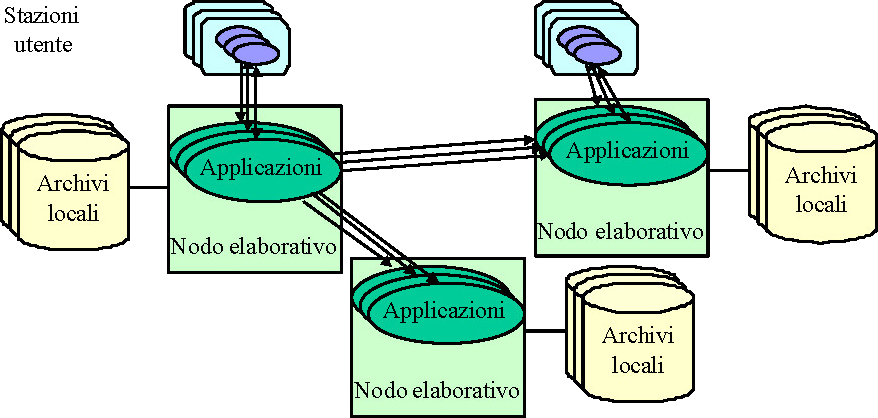
\includegraphics[width=0.50\textwidth]{images/sistemaDistr.png}
     }
     \hfill
     \subfloat[Sistema centralizzato\label{fig:sistemaCentr}]{%
       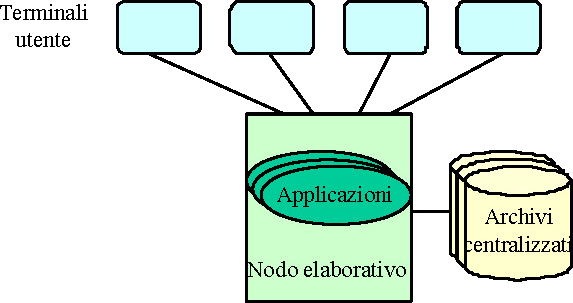
\includegraphics[width=0.50\textwidth]{images/sistemaCentr.png}
     }
     \caption{Differenza tra sistema distribuito e centralizzato.}
  	 \label{fig:sistemaDisCent}
\end{figure}
L'applicazione creata è eseguita su un sistema distribuito questo perché abbiamo bisogno di tempi di risposta bassi ed alta affidabilità dei dati. Per questo motivo il codice viene partizionato in piccoli problemi ed eseguiti dai nodi del nostro cluster. Il processo di partizione dei dati viene automatizzato dal framework Spark [\ref{sec:spark}] che si occupa della gestione, invio e recupero dei dati tra i vari nodi. 

\subsection{Caratteristiche di un sistema distribuito}
\label{subsec:caratteristiche di un sistema distribuito}
Un sistema distribuito si definisce tale se rispetta alcune caratteristiche come: 
\begin{itemize}
\item \textbf{Remoto}: le componenti di un sistema distribuito devono poter essere trattate allo stesso modo sia che siano in locale che in remoto.
\item \textbf{Concorrenza}: è possibile eseguire contemporaneamente due o più istruzioni su macchine differenti.
\item \textbf{Malfunzionamenti parziali}: Ogni componente del sistema può smettere di funzionare correttamente indipendentemente dalle altre componenti del sistema; questo non deve compromettere le funzionalità dell'intero sistema. I fallimenti che possono affliggere i processi possono essere di varia natura.
\item \textbf{Eterogeneità}: un sistema distribuito è eterogeneo per tecnologia sia hardware che software. Si realizza in tutti i contesti come rete di comunicazione, protocollo di rete, linguaggi di programmazione, applicazioni, etc.
\item \textbf{Autonomia}: un sistema distribuito non ha un singolo punto dal quale può essere controllato, coordinato e gestito. La collaborazione va ottenuta inviando messaggi tra le varie componenti del sistema e gestita tramite politiche di condivisione e di accesso che devono essere rigorosamente seguite. 
\item \textbf{Evoluzione}: un sistema distribuito può cambiare sostanzialmente durante la sua vita, sia perché cambia l'ambiente sia perché cambia la tecnologia utilizzata. L'obiettivo è quello di assecondare questi cambiamenti senza costi eccessivi.\cite{distSist:caratteristiche}
\end{itemize}

\subsection{Vantaggi e Svantaggi}
\label{subsec:vantaggi e svantaggi}
I sistemi distribuiti hanno dei pro e contro che sono da prendere in considerazione quando si vogliono adottare soluzioni di questo tipo.  
\\I vantaggi nell'utilizzo dei sistemi sono:
\begin{itemize}
\item \textbf{Connettività e collaborazione}: possibilità di condividere risorse hardware e software (compresi dati e applicazioni)
\item \textbf{Prestazioni e scalabilità}: la possibilità di aggiungere risorse, fornisce la capacità di migliorare le prestazioni e sostenere un carico che aumenta (scalabilità orizzontale)
\item \textbf{Tolleranza ai guasti}: grazie alla possibilità di replicare risorse e dati
\item \textbf{Apertura}: l'uso di protocolli standard aperti favorisce l'interoperabilità di hardware e software di fornitori diversi
\item \textbf{Economicità}: i sistemi distribuiti offrono spesso (ma non sempre) un miglior rapporto prezzo/qualità che i sistemi centralizzati basati su mainframe
\end{itemize}

Gli svantaggi invece sono:
\begin{itemize}
\item \textbf{Complessità}: i sistemi distribuiti sono più complessi di quelli centralizzati e quindi risultano più difficili da capire, inoltre, lo sviluppo delle applicazioni deve essere implementato ad hoc.
\item \textbf{Sicurezza}: l’accessibilità in rete pone problematiche di sicurezza
\item \textbf{Gestibilità}: è necessario uno sforzo maggiore per la gestione del sistema operativo e delle applicazioni
\end{itemize}

%\section{Stato d'arte}
\label{sec:stato d'arte}

\chapter{Overview e progettazione di sistema}
\label{chap:overview e progettazione di sistema}
In questo capitolo viene messo in luce lo scopo dell'elaborato realizzato con particolare attenzione alle scelte progettuali adottate e alle ricerche effettuate per implementare l'argomento trattato, onde presentare un quadro generale completo. Viene, inoltre, descritta l'architettura del software, sottolineando ed approfondendo le sue principali componenti.

\section{Scopo del progetto}
\label{sec:scopo del progetto}
Lo scopo principale del lavoro di tesi è quello di creare un sistema distribuito che permetta la visualizzazione real time, la storicizzazione e l'analisi delle transazioni  provenienti dalla blockchain di bitcoin. L'obiettivo, dunque, è quello di riuscire a creare un sistema che gestisca grandi quantità di dati in un ambiente distribuito, garantendo affidabilità e consistenza dei dati anche in caso di guasti.
\\Il sistema si rivolge ad un pubblico che vuole fare analisi delle transazioni processate dalla rete bitcoin. L'utente infatti, può controllare in real time le ultime transazioni elaborate, monitorare l'intera rete blockchain per risalire a tutta la catena di transazioni, oppure controllare gli hash (indirizzi) che hanno avuto maggior punteggio di PageRank.
\\Le ultime transazioni elaborate, hanno una serie di informazioni di dettaglio come il blocco di appartenenza, l'hash che ha generato quella transazione, il timestamp ed i destinatari dei bitcoin. Mentre per quanto riguarda il monitoraggiio dell'intera blockchain, l'utente può navigare con l'utilizzo del proprio mouse, in un grafo orientato rappresentante la storia di tutte le transazioni. Inoltre, il fruitore può controllare i nodi con il maggior punteggio di PageRank e localizzarlo all'interno del grafo.  

\section{Architettura  del progetto}
\label{sec:architettura del progetto}
Le principali scelte di progetto sono state prese coerentemente con lo stato dell'arte e si è tentato di non introdurre nuova complessità al panorama esistente, ricorrendo a tecnologie, protocolli e standard già esistenti ed affermati, senza definirne di nuovi. Quindi, l'architettura dovrà essere sufficientemente generale in modo da poter garantire nuovi sviluppi ed evoluzioni future e da non comportare l'esclusione a priori di determinate soluzioni e tecnologie. 
\\Il sistema, quindi, si divide logicamente in due moduli:
\begin{itemize}
	\item \textbf{Il Sistema distribuito (back-end)}: E' la parte non visibile all'utente. Si occupa del recupero dei dati dalla blockchain di bitcoin, della storicizzazione e della pubblicazione sui topic di kafka. Interamente scritto in Java, comprende Bitcoind, Spark, Hadoop, Neo4j, Zookeeper.
	\item \textbf{Webapp (front-end)}: E' la parte visibile all'utente finale. Si occupa della rappresentazione grafica delle transazioni. Scritto in principalmente in Javascript, utilizza la potenza di NodeJS per creare l'interfaccia grafica. Integra nel proprio ecosistema Express Handlebars, WebSocket, MaterialCSS e D3js.
\end{itemize}

\begin{figure}[H]
	\centering
	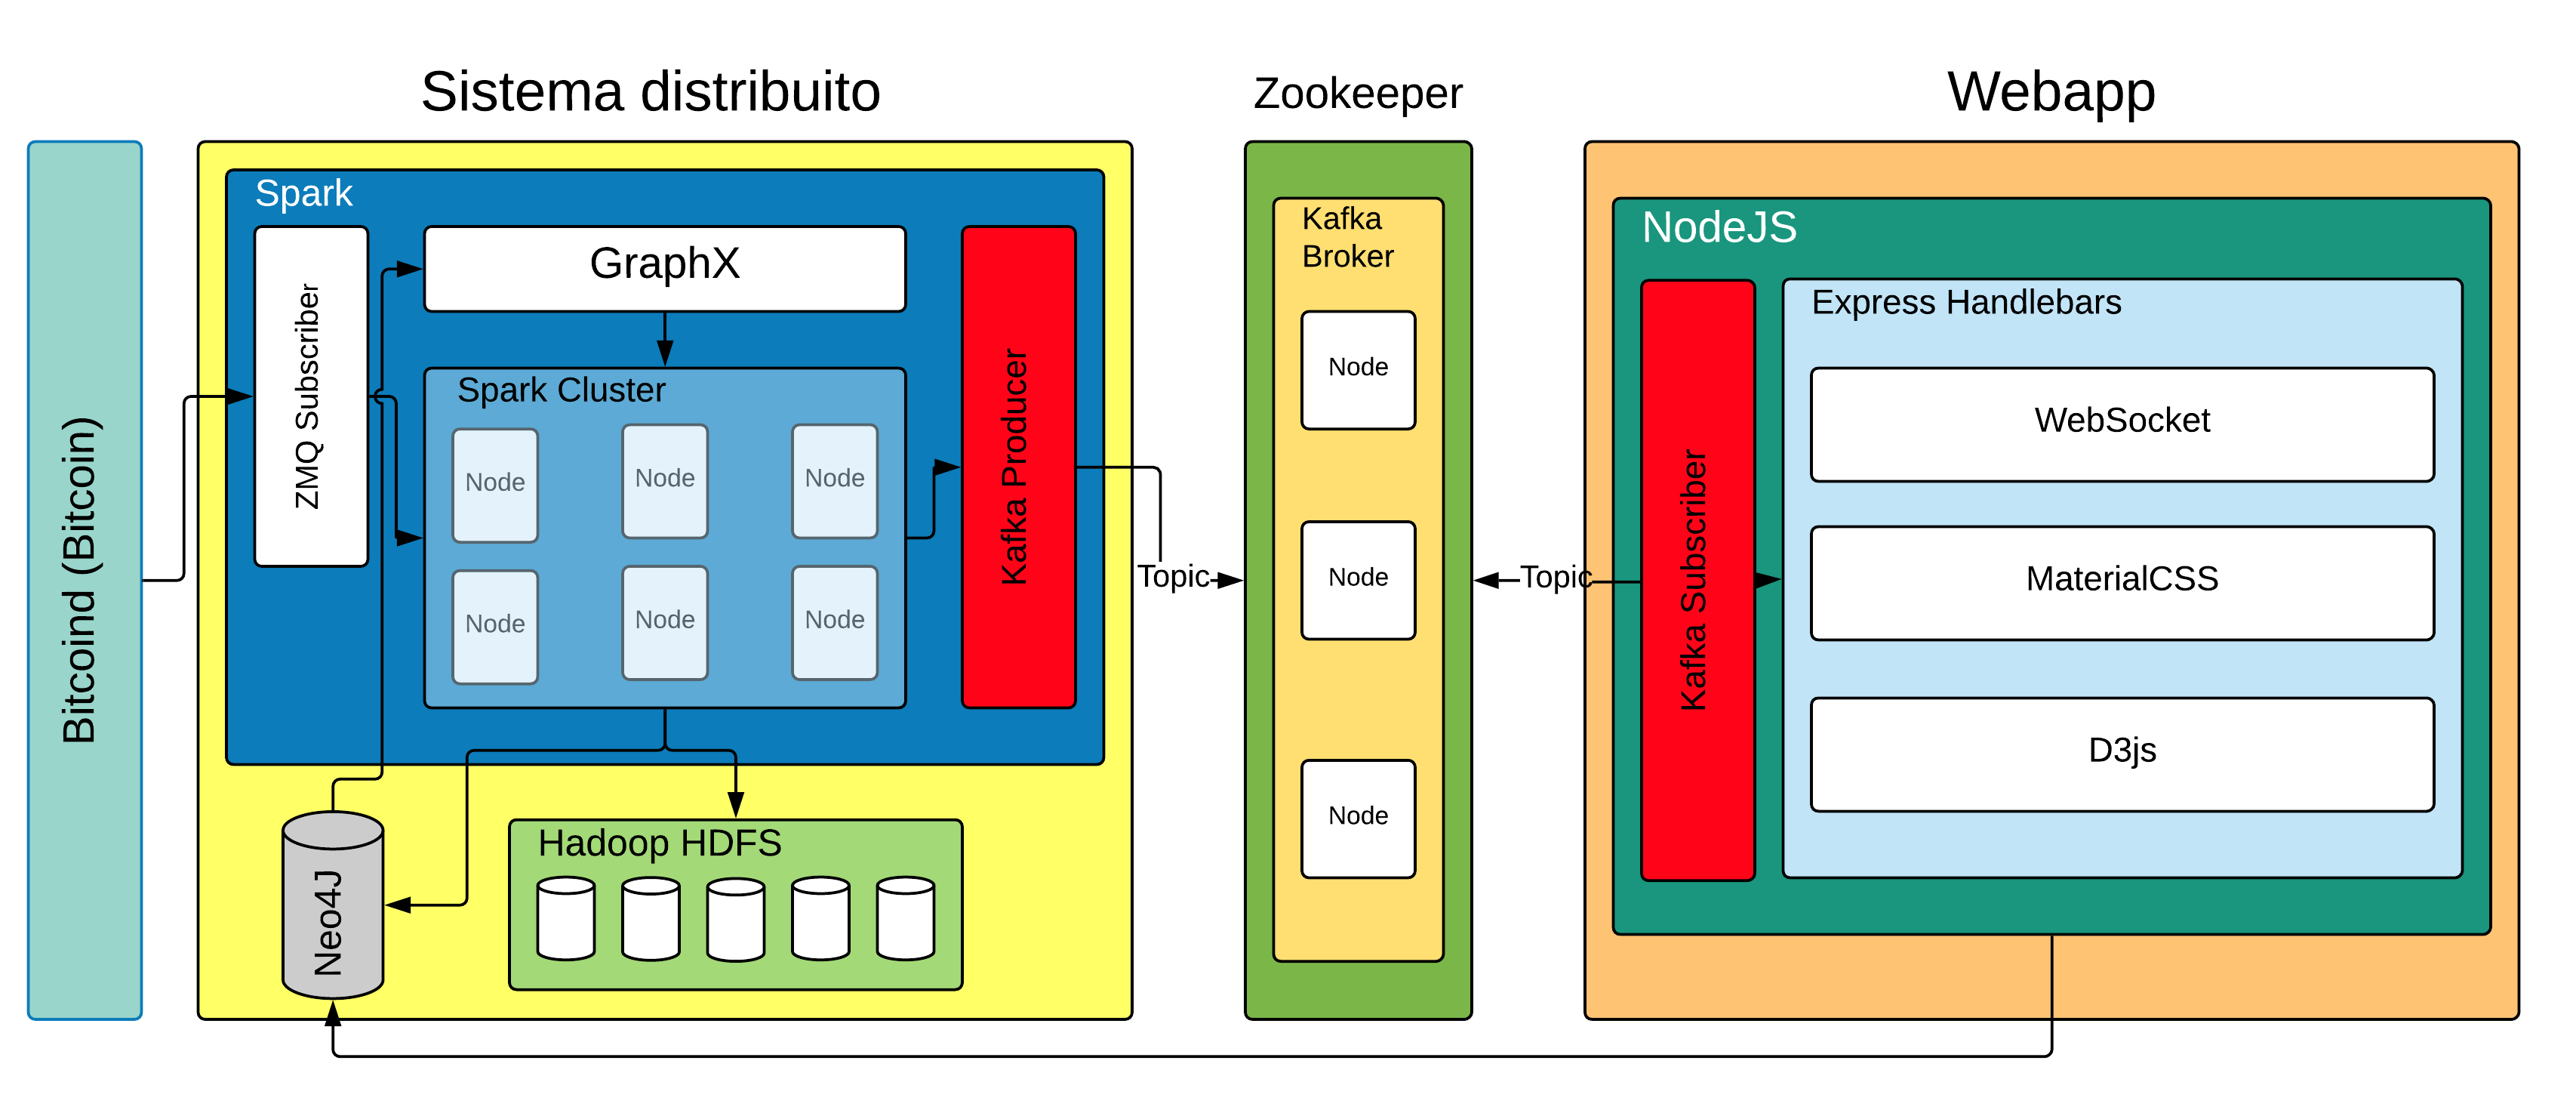
\includegraphics[width=\textwidth]{images/architetturaTesi.png}
	\caption{Architettura completa.}
	\label{fig:softwareArchitetture}
\end{figure}
 
Per la costruzione di questa infrastruttura, la prima grande sfida, è stata quella di trovare un framework o un tool che permettesse di creare e programmare su di un sistema distribuito, senza complicarci la vita. Facendo ricerche sul web, la tecnologia che più si accostava meglio al mio problema è stata Apache Spark [\ref{sec:spark}]. Questo strumento riesce a garantire a pieno i vincoli che ci siamo imposti, regalandoci la possibilità di creare un sistema distribuito su vari nodi impostando opportuni file di configurazione.
\\Risolto il problema infrastrutturale si è proceduto all'analisi dei singoli sottoproblemi. L'applicazione, per testare il carico di lavoro sul sistema, fa uso dei blocchi grezzi provenienti dal software nativo del progetto Bitcoin: Bitcoind [\ref{sec:bitcoind}]. Bitcoind è un demone che invia blocchi o transazioni (a seconda di come lo si imposta) su di una coda di tipo publisher-subscriber tramite protocollo ZeroMQ [\ref{sec:ZMQ}]. I dati, quindi, sono prelevati da Bitcoind grazie all'implementazione di un connettore creato ad hoc.
\\Ottenuti i blocchi dalla coda, è nata l'esigenza di conservare i dati ottenuti così da poterli processare ed analizzare. Fortunatamente, Spark offre una nativa collaborazione con il FileSystem distribuito Hadoop [\ref{sec:hadoop HDFS}], permettendomi di tenerli salvati su una memoria di massa distribuita.
\\Oltre ad Hadoop, i dati sono stati immagazzinati in Neo4j [\ref{sec:neo4j}]. Un database NoSQL che permette il salvataggio dei dati sottoforma di grafo, cosi da poter gestire facilmente i collegamenti tra le varie transazioni.
\\L'ultimo step, è stato quello di fare analisi delle transazioni, trovando i nodi con il maggior PageRank [\ref{sec:graphx (PageRank)}]. Anche in questo caso Spark è venuto in contro grazie al modulo GraphX, contenuto nel framework, il quale contiene algoritmi (come il PageRank) già sviluppati per l'analisi sui grafi.
\begin{figure}[H]
	\centering
	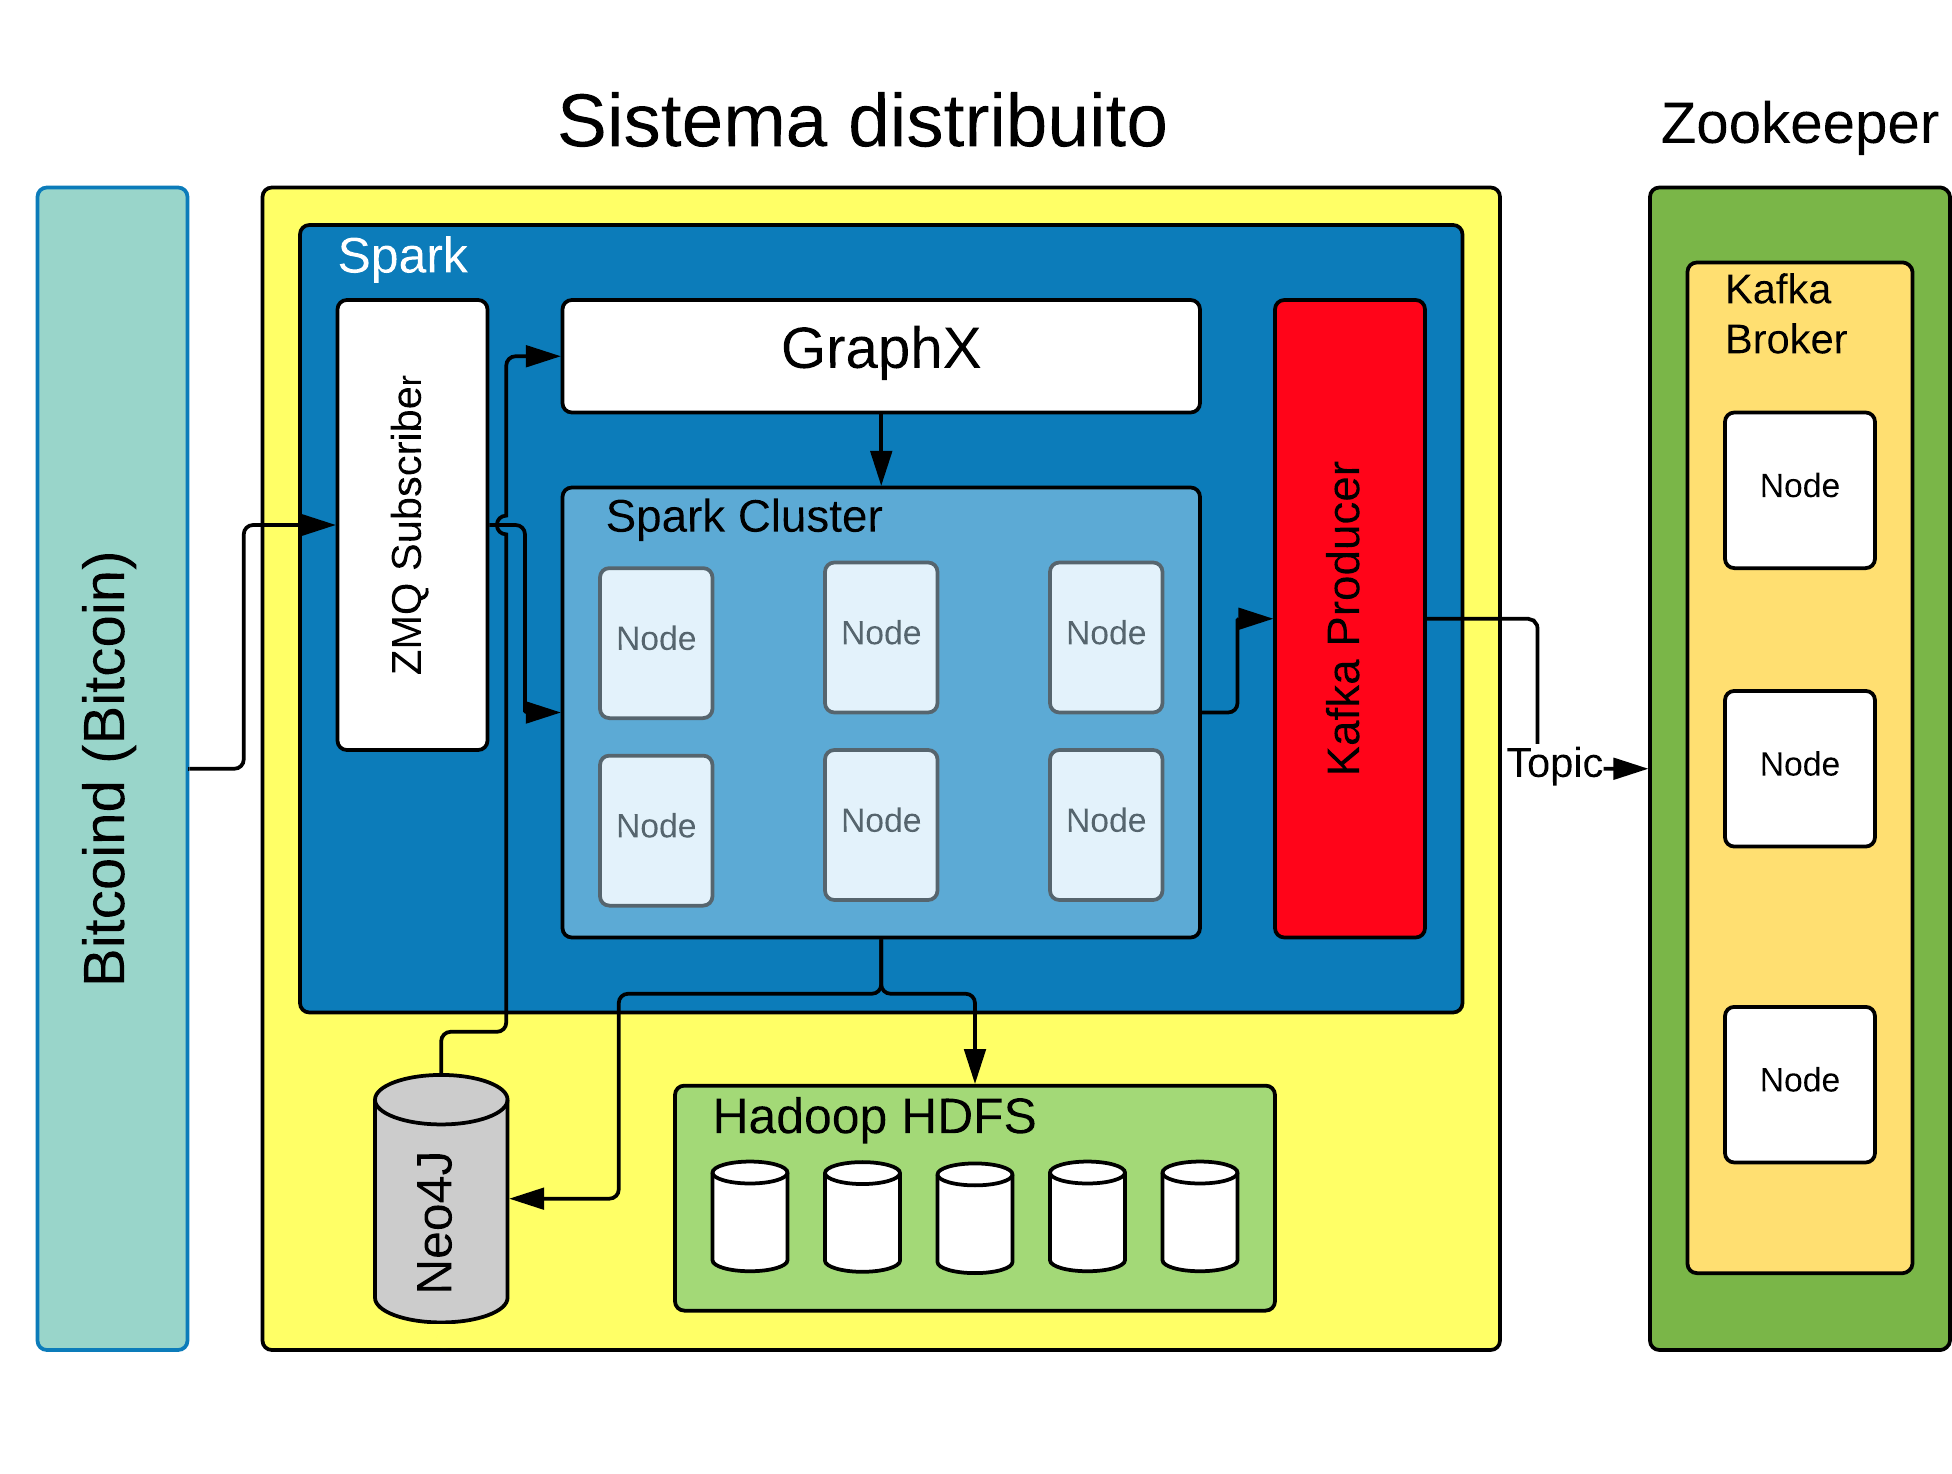
\includegraphics[width=\textwidth]{images/sistemaDistribuito.png}
	\caption{Architettura in dettaglio del sistema distribuito.}
	\label{fig:distribuitedSystemArchitetture}
\end{figure}  
Una volta che il sistema distribuito è completo, non resta che mostrare i risultati ottenuti. Le scelte nel campo del front-end sono migliaia ma per semplicità ed una forte attitudine ai sistemi real-time si è preferito usare NodeJS [\ref{sec:nodejs}]. NodeJS ha dei moduli che permettono l'accesso a Kafka, il tramite tra la parte di back-end e front-end. Quindi, con NodeJS è stato creato un sito web consentendo agli utenti dal proprio browser, di visualizzare lo stato delle transazioni, i valori del PageRank e le transazioni che arrivano in real time.
\begin{figure}[H]
	\centering
	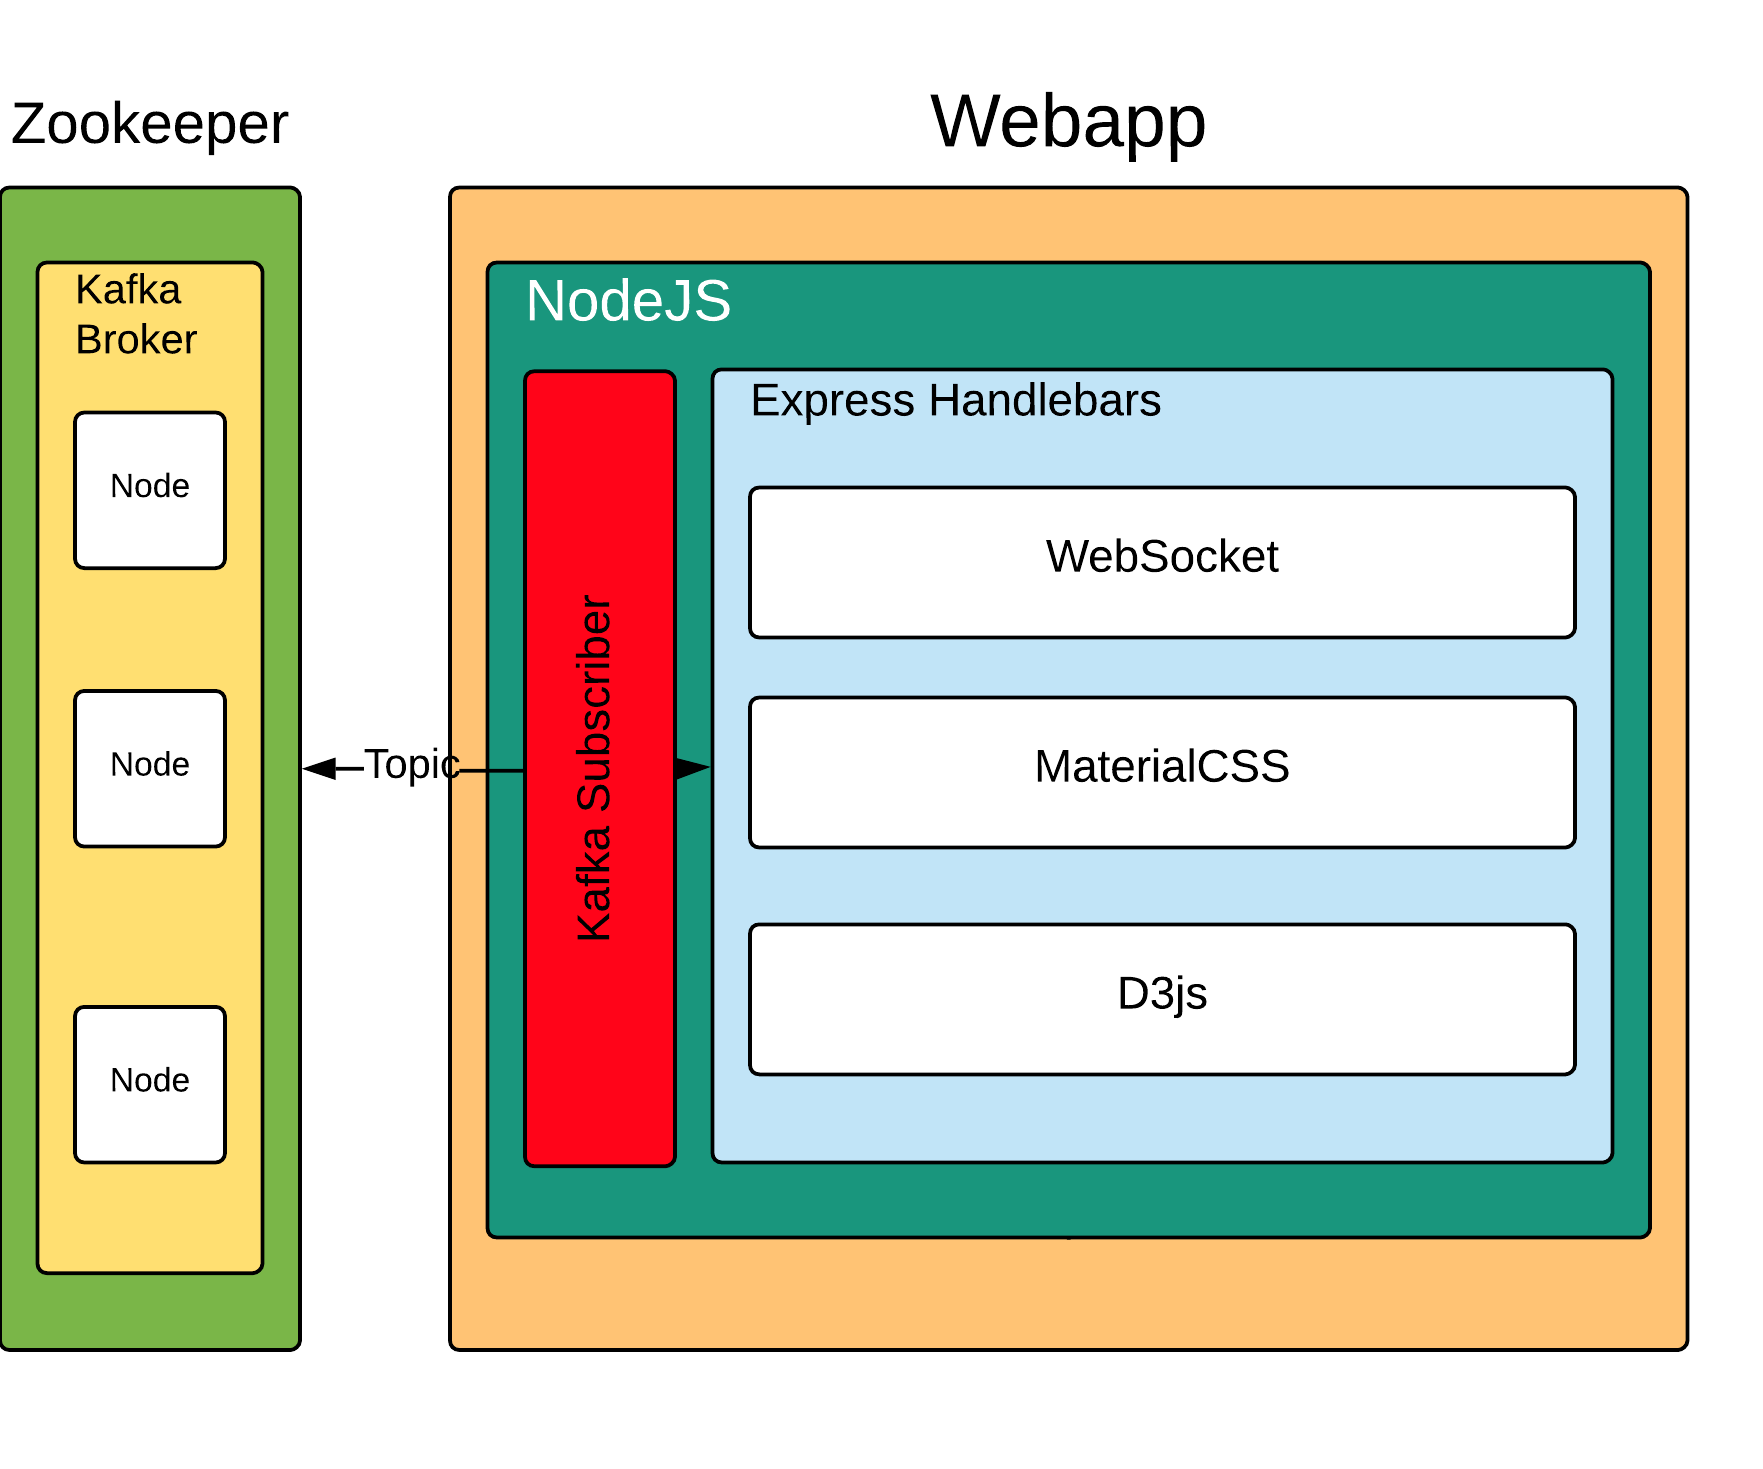
\includegraphics[width=\textwidth]{images/webApp.png}
	\caption{Architettura in dettaglio della webapp.}
	\label{fig:webAppArchitetture}
\end{figure}
\section{Sistema distribuito}
\label{sec:sistema distribuito}
\subsection{Bitcoind}
\label{sec:bitcoind}
Bitcoind è un software che implementa il protocollo Bitcoin per l'utilizzo delle remote procedure call(RPC). Esso è anche il secondo client Bitcoin nella storia del network.\cite{wiki:bitcoind}.
Questo programma è la fonte dei dati per l'applicazione, difatti invia i blocchi  


\subsubsection{ZMQ}
\label{sec:ZMQ}

\subsection{Apache Spark}
\label{sec:spark}
Apache Spark è un framework di calcolo del cluster per l'elaborazione di dati su larga scala, progettato e implementato nel 2010 da un gruppo di ricercatori dell’Università di Berkeley a San Francisco \cite{spark:hadoop}. Questo progetto nasce dall'esigenza di migliorare le prestazioni dei sistemi distribuiti “MapReduce”. Per questo si sviluppa il concetto di Resilient Distributed Dataset (RDD), che è la teoria alla base del sistema Spark. Un RDD rappresenta un set di dati che è suddiviso in partizioni (Una tabella chiave-valore suddivisa in tante sotto-tabelle o un file diviso in tanti segmenti). Un RDD ha la proprietà di essere immutabile, cioè una volta creato non può essere cambiato se non creandone un altro. La creazione di un RDD avviene a partire dai dati su disco (presi da HDFS) o da altre fonti di dati. Una volta creato, un RDD può restare in memoria oppure può essere materializzato su disco. Ogni RDD è descritto da un set completo di metadati che consentono la ricostruzione di una delle sue partizioni in caso di fault. Spark nasce come un sistema per creare e gestire job di analisi basati su trasformazioni di RDD. Dato che gli RDD nascono e vivono in memoria, l’esecuzione di lavori iterativi, o che trasformano più volte un set di dati, sono immensamente più rapide di una sequenza di MapReduce; questo perchè il disco non viene mai (o quasi mai) impiegato nell’elaborazione.
\\Come detto in precedenza, Spark non utilizza MapReduce come motore di esecuzione; invece, utilizza il proprio runtime distribuito (DAG) per l’esecuzione di jobs su un cluster. Quando viene invocata un’azione su un RDD, viene creato un “job”. Un Directed Acyclic Graph o DAG è un grafo aciclico in cui ogni nodo è una partizione di RDD e ogni vertice è una trasformazione. A differenza di MapReduce, il motore DAG di Spark può processare pipeline arbitrarie di operatori e tradurle in un unico “job” per l'utente.
\\Spark, infine, sta dimostrando di essere una buona piattaforma su cui costruire strumenti di analisi, infatti ha moduli per il Machine learning (MLlib), Elaborazione grafica (GraphX), Elaborazione di stream (Spark Streaming) ed SQL (Spark SQL) \cite{spark:hadoop}.
\begin{figure}[H]
	\centering
	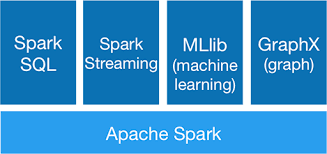
\includegraphics[width=\textwidth]{images/spark.png}
	\caption{Infrastruttura Spark.}
	\label{fig:sparkOverview}
\end{figure}
Nel sistema distribuito, poichè c'è l'esigenza di recuperare i dati in real time dalla coda di bitcoind, viene utilizzato Spark Streaming. Questo modulo è un'estensione dell'API Spark di base che consente l'elaborazione streaming, scalabile, ad alto throughput e con tolleranza agli errori dei flussi di dati in tempo reale. I dati, che possono provenire da diverse fonti, sono elaborati utilizzando algoritmi complessi espressi con funzioni di alto livello come \textit{map}, \textit{reduce}, \textit{join} e \textit{window}. I dati processati, infine possono essere inviati a filesystem (Hadoop) o database (Neo4j) per il salvataggio oppure ad altri moduli di Spark, dediti all'analisi, tipo machine learning (MLlib) o graph processing (GraphX). 
\\Internamente, Spark Streaming riceve streams di dati di input e li divide in batch, che vengono quindi elaborati dal motore Spark per generare il flusso finale di risultati. Per consentire il facile utilizzo di questi dati, fornisce un'astrazione di alto livello chiamata stream discretizzato o DStream, che rappresenta un flusso continuo di dati. E' possibile creare Dstreams da flussi di dati di input da sorgenti come Kafka, Flume e Kinesis o applicando operazioni di alto livello su altri Dstreams \cite{spark:home-streaming}. Internamente, un Dstream è rappresentato come una sequenza di RDD sulla quale possono essere effettuate le operazioni descritte in precedenza.
\begin{figure}[H]
	\centering
	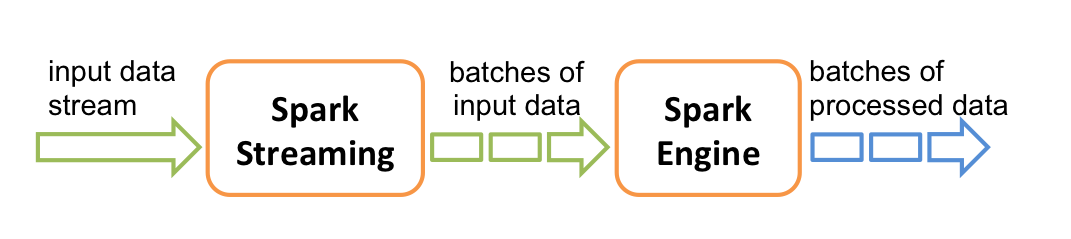
\includegraphics[width=\textwidth]{images/streamingSpark.png}
	\caption{Come vengono gestiti i dati in Spark Streaming.}
	\label{fig:streamingSpark}
\end{figure}
Nel sistema distribuito, per fare analisi dei dati provenienti dall'elaborazione di Spark, è stato scelto il modulo interno GraphX.
\\GraphX è un nuovo componetene di Apache Spark per grafi ed il calcolo parallelo (PageRank) su di essi. Estende gli RDD di spark introducendo gli Resilient Distribuited Property Graph, oggetti simili a grafi che permettono l'inserimento di proprietà per vertici e archi, rendendo facilitata l'implementazione. Inoltre, per aiutare nell'analisi, espone un insieme di operatori fondamentali (sottografo, joinVertices e aggregateMessages) come variante ottimizzata dell'API Pregel. In più, Graphx include una crescente collezione di algoritmi e costrutti per grafi per semplificare le attività di analisi \cite{spark:graphx}. Attualmente le sue API sono scritte in Scala, Java e Python.
\begin{figure}[H]
	\centering
	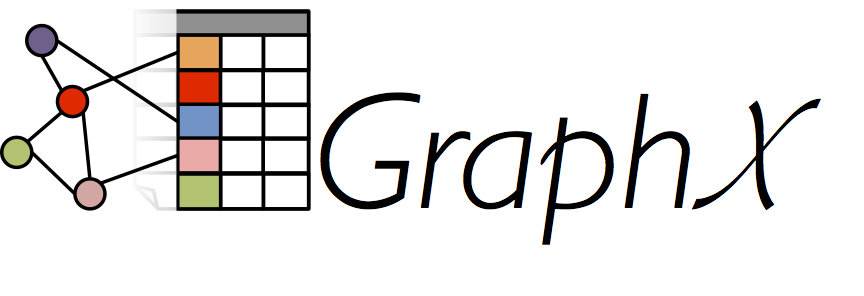
\includegraphics[width=\textwidth]{images/graphxLogo.png}
	\caption{Logo GraphX.}
	\label{fig:graphxLogo}
\end{figure}
GraphX, come detto in precedenza, gestisce i dati in memoria come se fossero grafi. Infatti, utilizza archi e vertici che hanno delle proprietà  connesse. Ogni vertice possiede un identificativo univoco a 64bit (VertexID), mentre, allo stesso modo, gli archi contengono gli identificativi di origine e partenza. Queste proprietà sono definite e tenuti in memoria come oggetti e di conseguenza con metodi creati ad-hoc per gestirli.  


\subsection{Hadoop HDFS}
\label{sec:hadoop HDFS}

\subsection{Neo4j}
\label{sec:neo4j}



\subsection{Zookeeper}
\label{sec:zookeeper}

\subsubsection{Kafka}
\label{sec:kafka}

\section{WebApp}
\label{sec:webapp}
Una applicazione web è una applicazione client/server per un ambiente stateless, cioè senza memoria, che utilizza le tecnologie internet. Con il termine Webapp si descrive un'applicazione accessibile via web per mezzo di una network, come ad esempio una Intranet o attraverso la rete Internet. Pertanto, saper programmare per il web significa conoscere i diversi meccanismi e strumenti per conservare o passare i dati, detti parametri, tra le diverse pagine dell'applicazione web. In pratica una Web-application, è un programma che non necessita di essere installato nel computer in quanto esso si rende disponibile su un server in rete e può essere fatto funzionare attraverso un normale Web browser (es. Google Chrome, Mozilla Firefox, Opera, ecc.). I client, dopo aver instaurato una connessione con il server, invia la richiesta per un servizio; il server dopo aver elaborato i dati necessari rende disponibile al client il servizio richiesto. A differenza dei siti web statici (HTML), l'applicazione web viene realizzata con una o più tecnologie (Javascript, Ajax, Servlet, Database ecc.) che permettono la creazione di un sito dinamico, cioè di un sito nel quale il contenuto delle pagine varia durante l'interazione.
\\Le applicazioni Web si pongono come valida alternativa alle tradizionali applicazioni Client/Server per vari motivi:
\begin{itemize}
\item \textit{Facilità di distribuzione e aggiornamento}: un'applicazione Web risiede interamente sul server, per cui la sua pubblicazione coincide con la distribuzione e l'aggiornamento ed è automaticamente disponibile a tutti gli utenti.
\item \textit{Accesso multi-piattaforma}: l'accesso all'applicazione è indipendente dall'hardware e dal sistema operativo utilizzato dagli utenti;
\item \textit{Riduzione del costo di gestione}: l'uso di Internet come infrastruttura per un'applicazione Web riduce notevolmente sia i costi di connettività che i costi di gestione dei client;
\item \textit{Scalabilità}: un'applicazione Web ben progettata può crescere insieme alle esigenze dell'azienda senza particolari problemi;
\end{itemize}
Per poter mostrare l'elaborazione di Spark nel sistema distribuito, si è preferito utilizzare una webapp per i motivi sopra citati. Questa applicazione web fa uso di tecnologie di ultima generazione quali NodeJs ed HTML5. Questo la rende fruibile a tutti gli utenti provvisti di Pc, Tablet o Smartphone con un browser installato. Nel seguente capito dunque vengono messi in luce i principali componenti che compongono la webapp, mostrando i punti forti di ogni tecnologia.
\begin{figure}[H]
	\centering
	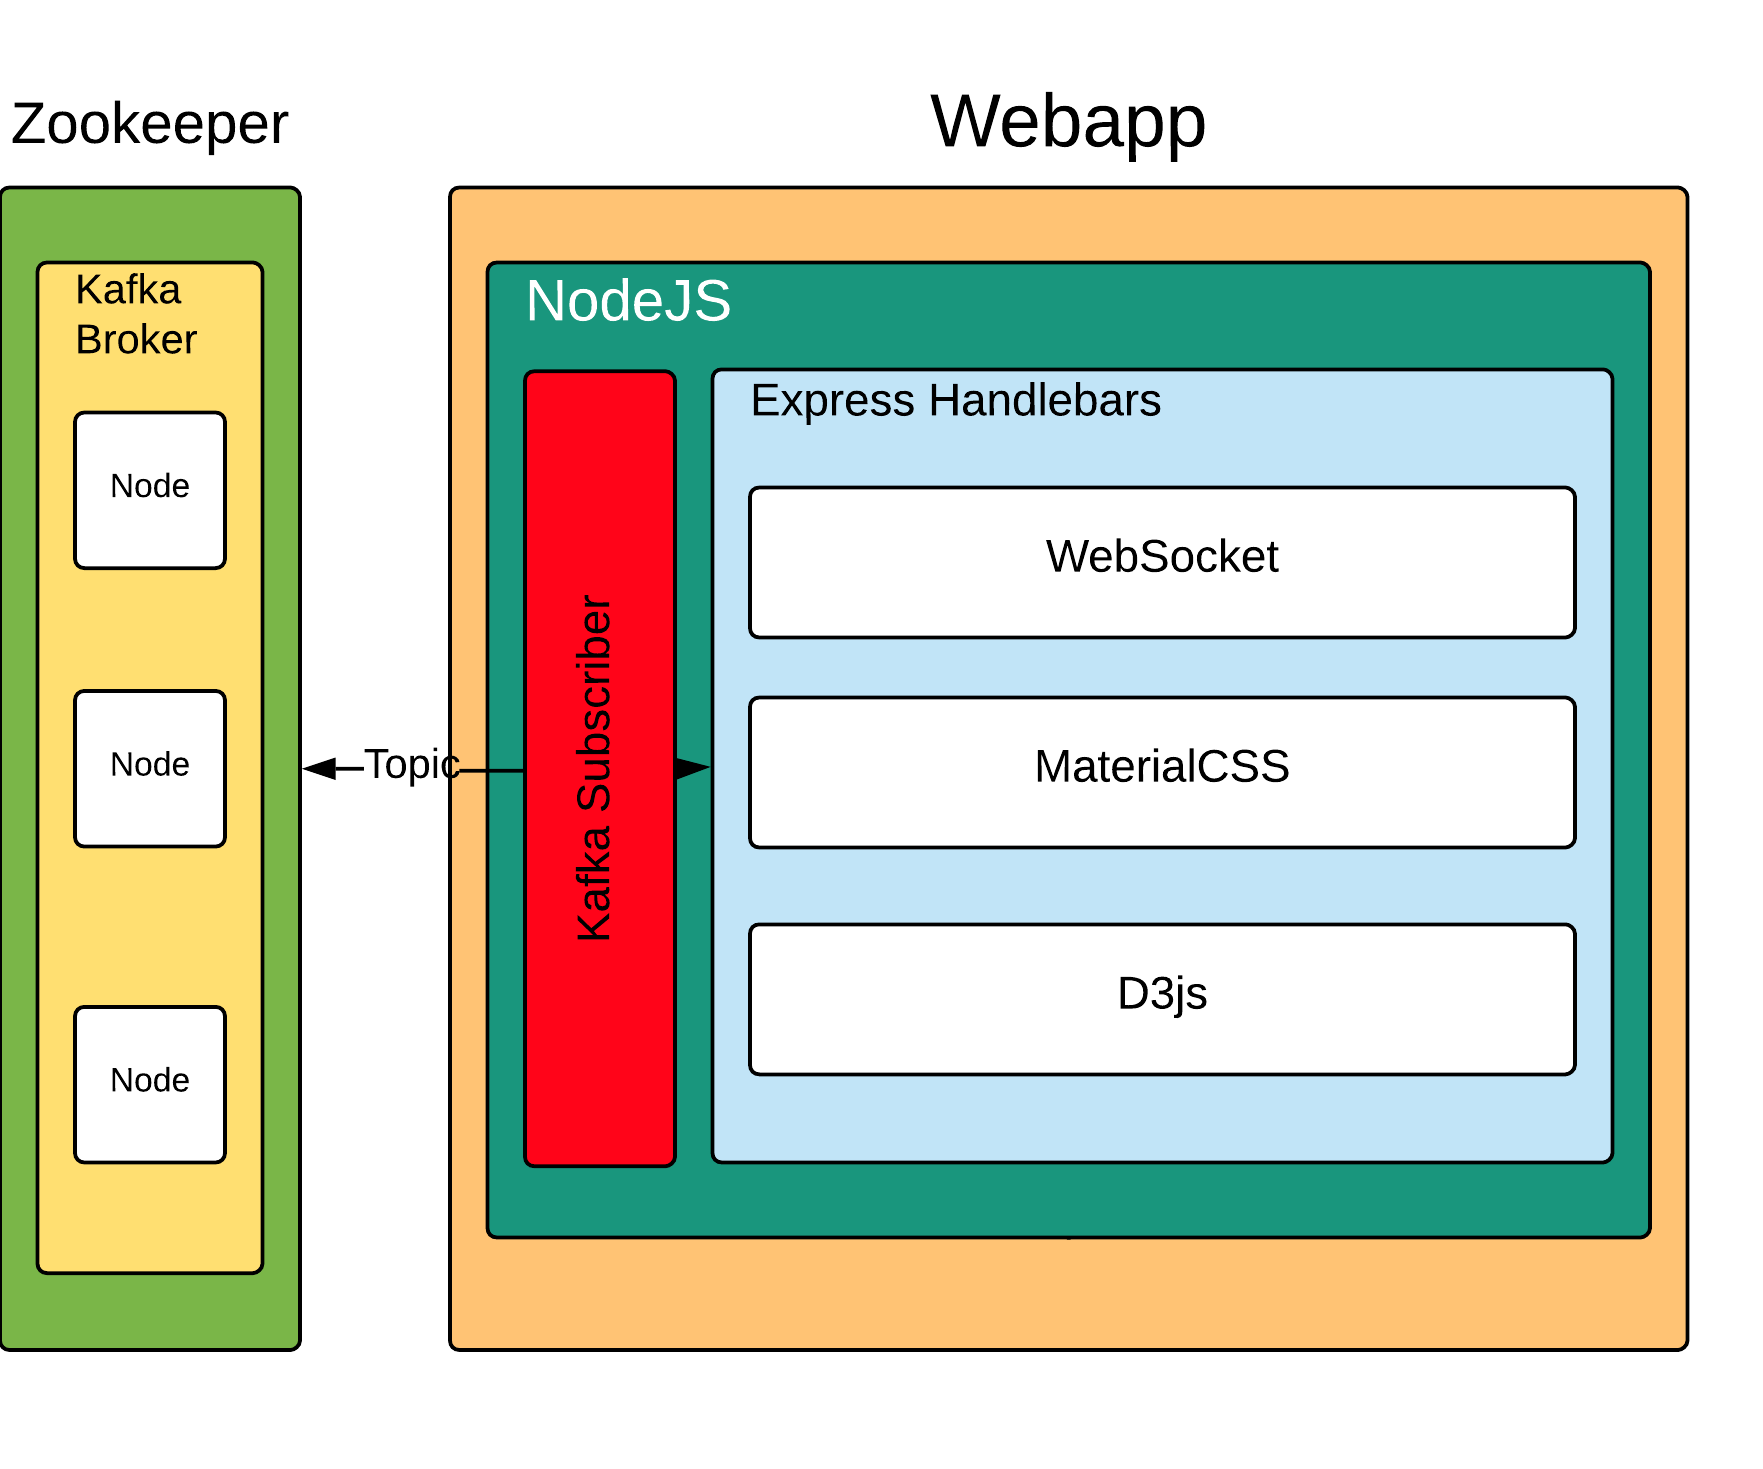
\includegraphics[width=\textwidth]{images/webApp.png}
	\caption{Architettura in dettaglio della webapp.}
	\label{fig:webAppArchitetture}
\end{figure}
\subsection{Node.js}
\label{sec:nodejs}
Node.js (anche conosciuto come Node o Nodejs) è un framework/piattaforma molto potente basato sul motore \textit{JavaScript V8} di Google Chrome, per creare facilmente applicazioni di Web veloci e scalabili. Pubblicata da Ryan Dahl nel 2009, viene utilizzato per sviluppare applicazioni Web intensive di I/O come siti di streaming video, applicazioni a pagina singola e altre applicazioni Web. Node.js è un ambiente open source, multi-piattaforma per lo sviluppo di applicazioni lato server completamente gratuito, utilizzato da migliaia di sviluppatori in tutto il mondo. Le applicazioni Node.js sono scritte in Javascript e possono essere eseguite all'interno del runtime di Node.js su OSX, Microsoft Windows e Linux. 
\\Utilizza un modello I/O non bloccante e basato sugli eventi che lo rende leggero ed efficiente, perfetto per applicazioni in tempo reale ad alta intensità di dati che funzionano su dispositivi distribuiti \cite{node:home}. Il modello di networking su cui si basa Node.js non è quello dei processi concorrenti, ma I/O event-driven: ciò vuol dire che Node richiede al sistema operativo di ricevere notifiche al verificarsi di determinati eventi, e rimane quindi in sleep fino alla notifica stessa. Solo in tale momento torna attivo per eseguire le istruzioni previste nella funzione di \textit{callback}, così chiamata perché da eseguire una volta ricevuta la notifica, che il risultato dell'elaborazione è disponibile. Tale modello di networking, implementato anche nella libreria Event machine per Ruby e nel framework Twisted per Python, è ritenuto più efficiente nelle situazioni critiche in cui si verifica un elevato traffico di rete \cite{node:wiki}. Di fronte alle esigenze di migliorare le performance dei software di rete Ryan Dahl ha creato una piattaforma che esegue le operazioni di I/O particolarmente lente (comunicazioni di rete o accesso al disco) in modo asincrono, rendendo la programmazione su Node JS diversa da qualsiasi esperienza con altri linguaggi. In definitiva, l'obiettivo di Node.js è quello di fornire un modo veloce per realizzare applicazioni web scalabili in termini di gestione delle connessioni da parte dei client verso il web server.
\\Nel momento in cui una operazione di I/O considerata lenta (di solito lo è se riguarda la rete o il disco fisso) viene eseguita da un programma in Node JS, V8 si occupa di trasferire la chiamata su un thread non bloccante fra quelli che ha a disposizione nella sua \textit{thread-pool base}. In questo modo, il thread principale con il codice può continuare la sua esecuzione senza context switch. Nel momento in cui una operazione collegata ai thread non bloccanti è terminata il kernel segnala che questo thread può tornare in coda di esecuzione. A questo punto però V8 si occuperà di intercettare il messaggio, mettere nella propria coda di esecuzione la funzione di callback specificata con l'operazione di I/O terminata e di rimettere il thread non bloccante a disposizione per altre operazioni di I/O. Così facendo, virtualmente il thread che esegue codice non si ferma mai, avvicendando le funzioni di callback delle varie operazioni terminate [\ref{fig:nodeEvent}].
\begin{figure}[H]
	\centering
	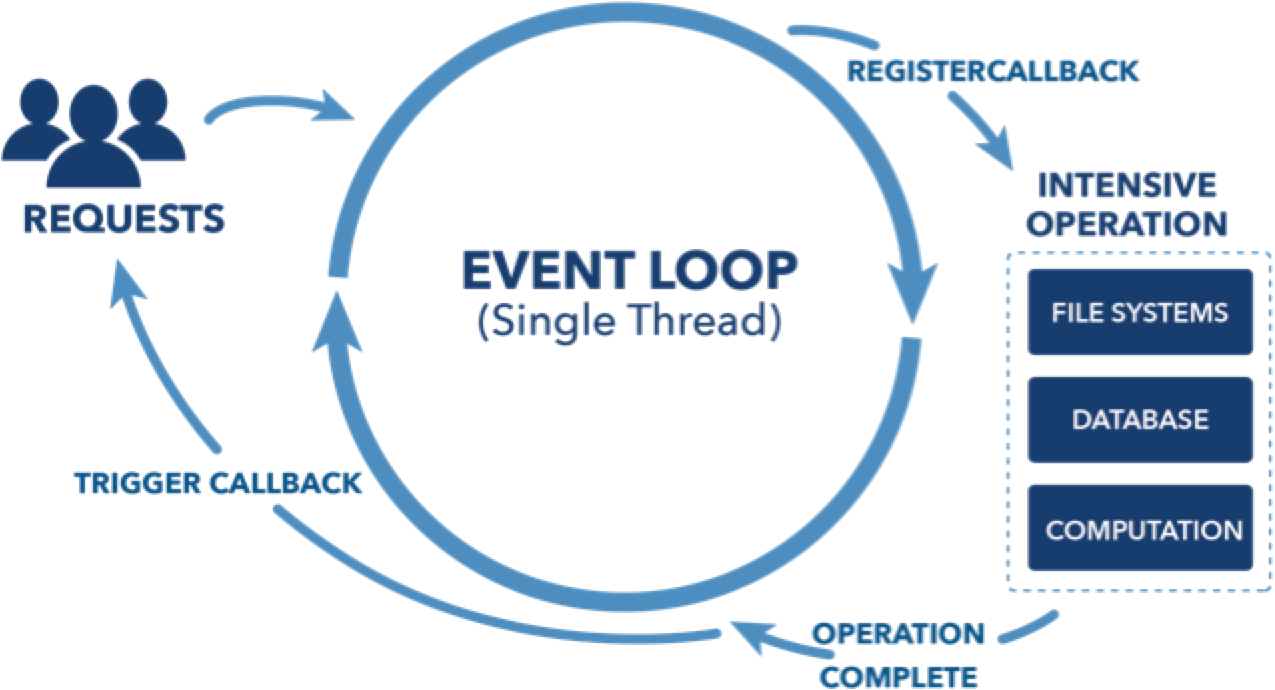
\includegraphics[width=\textwidth]{images/nodeEvent.png}
	\caption{Gestione eventi con Node.js.}
	\label{fig:nodeEvent}
\end{figure}
Bisogna però sempre tenere a mente, quando si progetta di scrivere un programma con Node.js, che questa architettura ha un effetto collaterale molto pesante; le operazioni che occupano per lungo tempo il thread in cui viene eseguito il codice (operazioni di calcolo onerose) bloccano l'interno software. Per questo motivo Node.js è assolutamente sconsigliato in caso di operazioni di calcolo complesse e nella fase di progettazione di programmi che usano questa piattaforma è sempre necessario utilizzare questa caratteristica come criterio fondamentale per la scrittura del codice.
Di seguito sono alcune delle caratteristiche importanti che rendono Node.js la prima scelta di architetti del software:
\begin{itemize}
\item \textbf{Asynchronous and Event Driven}: Tutte le API della libreria Node.js sono asincrone, ovvero non bloccanti. Significa essenzialmente che un server basato su Node non aspetta mai che un'API restituisca i dati. Il server passa all'API successiva dopo averlo chiamato ed un meccanismo di notifica di eventi consente al server di ottenere una risposta dalla precedente chiamata.
\item \textbf{Molto veloce}: Essendo costruito sul motore Javascript V8 di Google Chrome, Node.js è molto veloce nell'esecuzione del codice.
\item \textbf{Thread singolo ma altamente scalabile}: Node utilizza un singolo thread con loop di eventi. Il meccanismo degli eventi aiuta il server a rispondere in modo non bloccante e rende il server altamente scalabile rispetto ai server tradizionali che creano thread limitati per gestire le richieste. Quindi, Node utilizza un singolo programma con thread e lo stesso programma può fornire il servizio a un numero molto più grande di richieste rispetto ai server come Apache HTTP Server.
\item \textbf{Nessun Buffering}: Le applicazioni create con node non bufferizzano mai alcun dato. Queste applicazioni generano semplicemente i dati in blocchi.
\item \textbf{Licenza}: Node è rilasciato sotto licenza MIT. 
\end{itemize}
Esiste un mondo attorno a Javascript composto da librerie che ne estendono le funzionalità. Stesso discorso vale per Node.js, in quanto è attiva una comunità di sviluppo che ha realizzato in questi anni molte librerie per realizzare particolari tipi di supporto (database, Network, . . . ) ed un sistema di installazione di questi moduli che si occupa anche di eventuali dipendenze: \textit{npm}. Nei prossimi capitoli saranno analizzati alcuni progetti legati a Node.js usati nella creazione della webapp.

\subsubsection{Express.js ed Handlebars}
\label{sec:express handlebars}
Express.js (anche chiamato semplicemente Express) è un framework basato su Node.js che offre un insieme robusto di utilità per realizzare agilmente un'architettura \textit{MVC (Model-View-Controller)} sul lato server di applicazioni web single-page, multi-page ed ibride.
\\Basato sul modulo di Node chiamato \textit{connect}, risulta essere un ottimo "connettore" o \textit{middleware} tra le diverse librerie che possono popolare una webapp, tra cui WebSocket, Passport, Mustache.js, Handlebars, etc.
\\Le funzionalità offerte sono il \textit{routing}, la possibilità di gestire le configurazioni dell'applicazione ed un motore di templating.
\\Al centro di questa libreria c'è il concetto di flusso di funzioni, o come piace dire a certe persone, un set di \textit{livelli di funzione}. Infatti, per creare un'applicazione Express c'è bisogno di creare una sequenza di funzioni (livelli) che il framework può navigare. 
\\Quando una di queste decide di entrare in gioco, può completare il processo e fermare la sequenza. Dopodiché Express riprende a scorrere la sequenza fino alla fine.
\\Queste funzioni hanno delle callback associate che sono eseguite nel momento in cui un client effettua una richiesta. Questo processo prende il nome di Routing.
\\Il routing, dunque, è una funzionalità di Express.js, che determina la risposta ad una richiesta client ad un endpoint particolare; il quale può essere un URI (o percorso) o un metodo di richiesta HTTP specifico. In pratica, con Express, si possono gestire le richieste e le risposte \textit{in the middle}, cioè fra server e client. Quando il server riceve una richiesta HTTP la racchiude all'interno di un oggetto \textit{ServerRequest}. Questo oggetto, insieme all'oggetto \textit{ServerResponse}, viene passato al primo middleware che ne può modificare il contenuto, o aggiungere proprietà. Una volta terminata la modifica, il middleware richiamerà il successivo nell'eventuale catena (di funzioni) presente.
\begin{figure}[H]
	\centering
	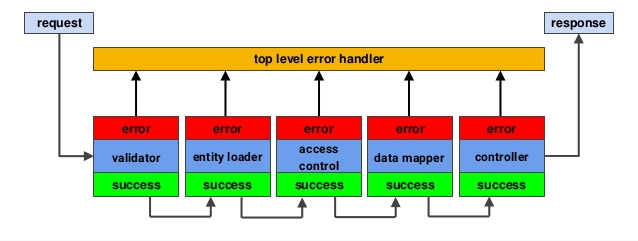
\includegraphics[width=\textwidth]{images/ExpressRoute.png}
	\caption{Visualizzazione della catena di funzioni per rispondere ad una richiesta}
	\label{fig:expressFlow}
\end{figure}
Se l'ultima funzione della catena deve restituire un HTML come risultato, Express chiama in causa il \textit{template engine}. Questo motore, infatti si occupa di fare il tramite tra i dati presenti nel layer model e quello di presentazione. In particolare elabora la richiesta producendo, in fase di run-time, un HTML dinamico partendo da una struttura definita (template). Esistono diversi motori che possono essere utilizzati con Express ognuno con le proprie particolarità e specifiche. 
\\Per questo elaborato la scelta del templating engine è caduta su \textit{Handlebars.js}. La libreria di templating Handlebars consente di creare un'interfaccia utente ricca includendo HTML statico e contenuto dinamico, che possono essere specificati nelle doppie parentesi graffe. Handlebars.js è molto popolare, semplice da usare e con una grande community. È basato sul linguaggio dei modelli di Mustache, ma lo migliora in molti aspetti. Con Handlebars, si può separare la generazione di HTML dal resto del JavaScript e scrivere codice più pulito. Inoltre, aggiunge costrutti (if e cicli for) che permettono di creare dinamicamente l'HTML. Infine, introduce un sistema di \textit{partial} che permette allo sviluppatore di inserire nelle proprie pagine, porzioni di HTML provenienti da file esterni. 
\\Express, quindi, per costruire la pagina di risposta da inviare al client, chiama Handlerbars che preleva i file con estensione \textit{.handlebars} li "compila" e genera il risultato finale.

\begin{lstlisting}[language=HTML, label=lst:HandlebarsTemplate, caption={Esempio di HTML scritto con Handlebars.}]
<div class="entry">
  <h1>{{title}}</h1>
  <h2>By {{author.name}}</h2>
  <div class="body">
    {{body}}
  </div>
</div>
\end{lstlisting} 

Il listato \ref{lst:HandlebarsTemplate} è un esempio di HTML scritto con la sintassi di Hadelbars. I valori \textit{title}, \textit{author.name} e \textit{body} saranno sostituiti, in fase di run-time, con i valori provenienti dal controller che passerà un oggetto all'engine templating. vedi listato \ref{lst:handleCode}.

\begin{lstlisting}[language=Javascript, label=lst:handleCode, caption={Esempio di variabile passata dal controller al template engine.}]
var context = {
  title: "My First Blog Post!",
  author: {
    id: 47,
    name: "Yehuda Katz"
  },
  body: "My first post. Wheeeee!"
};
\end{lstlisting} 

\subsubsection{WebSocket}
\label{sec:WebSocket}
L'applicazione web dell'elaborato di tesi, come detto in precedenza, prevede una interfaccia grafica per la visualizzazione delle ultime transazioni provenienti da Bitcoin. Per poter implementare questa funzionalità, c'è bisogno di utilizzare tecniche che permettano l'invio di dati tra client e server. Dal semplice request/response di HTTP, l'evoluzione del web e delle sue tecnologie ha portato alla nascita di nuove tecnologie per migliorare sempre di più la comunicazione remota.
\\Il modello tradizionale di comunicazione, derivato dalle specifiche standard di HTTP, prevedeva una comunicazione sincrona: in seguito a una azione dell'utente (request), il server eseguiva l'operazione richiesta e restituiva il risultato (response). Dopo la richiesta iniziale, il client si poneva in uno stato di attesa fino a quando la risposta non era ricevuta, risultando in uno spreco di tempo e risorse. Il refresh della pagina peggiorava inoltre la user-experience. Allo stesso tempo, il server non manteneva nessuna informazione riguardo alla comunicazione appena avvenuta. Più richieste della stessa operazione dunque venivano ogni volta re-processate e rigenerate per ogni client che le richiedeva. Una comunicazione di questo tipo, semplice da effettuare dal punto di vista implementativo, risulta tuttavia inefficiente e inadatta ad applicazioni di larga scala moderne.
\\Il primo fondamentale passo è stato rendere la comunicazione da sincrona ad asincrona. Ciò è stato possibile attraverso l'uso di plugin esterni, come Flash, oppure tramite nuovi meccanismi come Ajax. Tuttavia, entrambi presentano dei problemi: nel primo caso, un utente poteva non aver intenzione di installare software esterno, rendendo così inutile il plugin; nel secondo caso, la gestione stessa della comunicazione attraverso Javascript poteva velocemente raggiungere livelli di complessità non accettabili per grandi applicazioni. Per questi motivi la comunicazione tra client e server distribuito, è implementata con l'utilizzo della nuova tecnologia associata ad HTML5: i \textit{WebSocket}.
Formalmente, WebSocket è una tecnologia web che fornisce canali di comunicazione full-duplex attraverso una singola connessione TCP. L'API del WebSocket è stata standardizzata dal W3C e il protocollo WebSocket è stato standardizzato dall'IETF come RFC 6455 \cite{websocket:wiki}.
\\Dunque, tra le novità portate da HTML5, i WebSocket rappresentano quella di maggior importanza dal punto di vista dell'interazione tra client e server. WebSocket è una tecnologia per effettuare comunicazioni bidirezionali in tempo reale. Essi prevedono un canale di comunicazione sempre attivo, a bassa latenza, tra client e server, utilizzabile da entrambi sia in scrittura che in lettura. Tale canale è costituito da una connessione TCP persistente, garantito da un handshaking client-key iniziale ed un modello di sicurezza originbased. Per la protezione dei dati trasmessi contro lo sniffing sono applicate apposite maschere. 
\\Le caratteristiche principali dei WebSocket:
\begin{itemize}
\item \textbf{Bidirezionali}: Quando il canale di comunicazione è attivo, sia il client che il server sono connessi ed entrambi possono inviare e ricevere messaggi.
\item \textbf{Full-duplex}: Dati inviati contemporaneamente dai due attori (client e server) non generano collisioni e vengono ricevuti correttamente.
\item \textbf{Basati su TCP}: Il protocollo usato a livello di rete per la comunicazione è il TCP, che garantisce un meccanismo affidabile (controllo degli errori, re-invio di pacchetti persi, ecc) per il trasporto di byte da una sorgente a una destinazione.
\item \textbf{Client-key handshake}: All'apertura di una connessione, il client invia al server una chiave segreta di 16 byte codificata con base64. Il server aggiunge a questa un'altra stringa, detta \textit{magic string}, specificata nel protocollo (“258EAFA5-E914-47DA-95CA-C5AB0DC85B11”), codifica con SHA1 e invia il risultato al client. Cosi facendo, il client può verificare che l’identità del server che ha risposto corrisponda a quella desiderata.
\item \textbf{Sicurezza origin-based}: Alla richiesta di una nuova connessione, il server può identificare l'origine della richiesta come non autorizzata o non attendibile e rifiutarla.
\item \textbf{Maschera dei dati}: Nella trama iniziale di ogni messaggio, il client invia una maschera di 4 byte per l'offuscamento. Effettuando uno XOR bit a bit tra i dati trasmessi e la chiave è possibile ottenere il messaggio originale. Ciò è utile per evitare lo sniffing, cioè l'intercettazione di informazioni da parte di terze parti.
\end{itemize}
\begin{figure}[H]
	\centering
	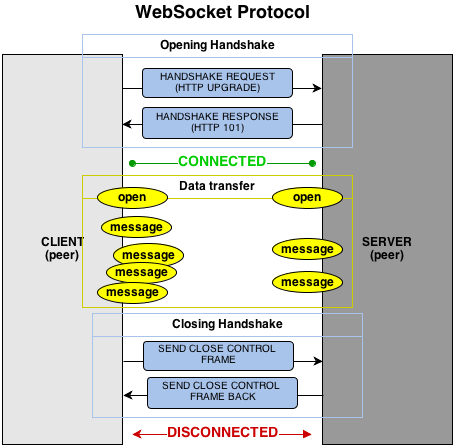
\includegraphics[width=\textwidth]{images/websocketProtocol.png}
	\caption{Comunicazione client/server tramite WebSocket}
	\label{fig:websocketProtocol}
\end{figure}
WebSocket è disegnato per essere implementato sia lato browser che lato server, ma può essere utilizzato anche da qualsiasi applicazione client-server. L'utilizzo dei WebSocket lato client, è possibile attraverso l'uso di specifiche API Javascript che consentono di ottenere informazioni sullo stato della connessione (aperta, chiusa, in apertura o in chiusura), di interagire con essa (inviare dati o chiudere la comunicazione) o di gestire particolari eventi come la ricezione di errori. Lato server, invece, esistono implementazioni dei WebSocket per la maggior parte dei linguaggi più utilizzati (Node.js, Java, C\#, Python, Ruby).

\subsubsection{MaterializeCSS}
\label{sec:materialCSS}
L'interfaccia grafica, \textit{GUI (Graphical User Interface)} o \textit{UI (User Interface)}, di una applicazione web determina, in molti casi, il suo successo. Progettare e programmare bene questo componente, quindi, ha un peso molto importante sulla buona riuscita anche del sistema sottostante che lo alimenta. 
\\Materialize CSS è una libreria che permette di creare interfacce in \textit{Material Design}. Creato e progettato da Google, Material Design è un linguaggio di progettazione che combina i principi classici del design di successo con l'innovazione e la tecnologia. L'obiettivo di Google è sviluppare un sistema di progettazione che consenta un'esperienza utente unificata su tutti i loro prodotti. Sebbene si possa scegliere tra milioni di librerie, la scelta di questo tool risulta molto promettente ed è una valida alternativa a prodotti affermati, quali Bootstrap o Foundation, con i quali è molto più complicato produrre un'interfaccia con una vera identità. MaterializeCSS dunque è un framework CSS usato per creare siti \textit{responsive}. Offre layout, animazioni e molti altri componenti che rendono semplice la creazione di pagine web.
\\Le principali caratteristiche sono:
\begin{itemize}
\item \textbf{Installazione}: L'installazione del framework è estremamente semplice, infatti bisogna solo importare i CSS e i javascript nel tag head nelle pagine html del proprio sito.
\item \textbf{Grid System}: Materialize divide il layout di un pagina web in 12 colonne. Questo sistema prende il nome di \textit{grid system} e permette di utilizzare classi \textit{container} che rendono il sito responsive e quindi utilizzabile su ogni dispositivo.
\item \textbf{Componenti}: Il framework ha una moltitudine di componenti \textit{pronti all'uso}. E' possibile   
\end{itemize} 

\subsubsection{D3.js}
\label{sec:d3js}
Ultimo componente di maggiore interesse è la libreria \textit{D3.js}. Questa libreria è usata all'interno di MaterilizeCSS per disegnare i grafi delle transazioni. D3.js (o solo D3 per Data-Driven Documents) è una libreria Javascript scritta da Mike Bostock come progetto successore di un precedente tool di visualizzazione chiamato Protovis. E’ basata sugli standard web e sfrutta appieno le tecnologie dei browser per manipolare gli elementi: come per JQuery, si utilizza la sintassi CSS per i selettori e si applicano gli stili agli elementi tramite fogli CSS. D3 a differenza delle altre librerie di grafici, non offre un insieme di grafici già pronti all'uso, bensì un potente framework che permette di realizzare praticamente qualsiasi tipo di grafico manipolando gli elementi di una pagina web di tipo HTML, SVG o Canvas in base al contenuto di un dataset.
\\La libreria JavaScript D3, incorporata in una pagina web HTML, utilizza funzioni JavaScript prefatte per selezionare elementi del DOM, creare elementi SVG, aggiungergli uno stile grafico, oppure transizioni, effetti di movimento e/o tooltip. Questi oggetti posso essere largamente personalizzati utilizzando lo standard web dei "fogli di stile a cascata", chiamati in inglese CSS. In questo modo grandi collezioni di dati possono essere facilmente convertiti in oggetti SVG usando semplici funzioni di D3 e così generare ricche rappresentazioni grafiche di numeri, testi, mappe e diagrammi. I dati utilizzati possono essere in diversi formati, il più comune è il JSON, valori separati da virgola CSV o geoJSON, ma, se necessario, di possono scrivere funzioni JavaScript apposta per leggere dati in altri formati. Il concetto centrale del design di D3 è permettere al programmatore di usare dei selettori, come per i CSS, per scegliere i nodi all'interno del DOM Document Object Model e quindi usare operatori per manipolarli, similmente alla libreria jQuery (see Bostock, Ogievetsky e Heer, chap. 3). La selezione può essere basata su tag (come nell'esempio qui sopra), elementi, classi, identificatori, attributi o punti della gerarchia. Una volta che gli elementi sono selezionati possiamo applicare operazioni su di essi. Questo comprende leggere ed impostare attributi, mostrare testi, formattare. Gli elementi possono anche essere aggiunti e rimossi. Questo processo di modifica, creazione ed eliminazione di elementi HTML, può essere eseguito in base ai set di dati forniti, che è il concetto di base di D3.js.
\chapter{Scelte tecniche ed implementazione}
\label{chap:implementazione}
Data la natura dell'elaborato, ossia il recupero e l'analisi delle transazioni provenienti da Bitcoin, si è deciso di implementare una soluzione che prevede i seguenti progetti:
\begin{itemize}
\item \textbf{Sistema Distribuito (SD in futuro)}: Applicazione distribuita che implementa la parte back-end;
\item \textbf{Blockchain Explorer}: applicazione web che implementa il componente front-end.
\end{itemize}
Le due applicazioni sono sviluppate con tecnologie e linguaggi diversi. In questo capitolo, viene esposta l'implementazione dei software, attraverso porzioni di codice  che aiuteranno a capire al meglio come le due applicazione cooperano nel raggiungimento dell'obiettivo finale.
\\ I linguaggi utilizzati per sviluppare i progetti sono Java 8 per la parte Beck-end , Javascript e HTML5 per la parte front-end.
\begin{itemize}
\item \textbf{Java 8}: Questo linguaggio orientato agli oggetti, è il più diffuso al mondo grazie alla sua portabilità. Infatti permette di scrivere codice in grado di essere eseguito indipendentemente dalla piattaforma e quindi sui principali sistemi operativi quali Microsoft, Linux e macOS. Questa peculiarità rende Java uno tra i più famosi linguaggi conosciuti e distribuiti al mondo.
\\Java ha le seguenti caratteristiche che lo rendono unico nel suo genere:
\begin{itemize}
\item \textbf{Orientato agli oggetti}: In Java, tutto è un oggetto. Java può essere facilmente esteso poiché si basa sul modello Object.
\item \textbf{Platform Independent}: A differenza di molti altri linguaggi di programmazione, Java viene compilato in un codice byte indipendente dalla piattaforma. Questo codice viene distribuito sul web e interpretato dalla Virtual Machine (JVM) su qualsiasi piattaforma su cui viene eseguito.
\item \textbf{Semplice}: Java è progettato per essere facile da imparare, perchè si basa sul concetto della programmazione orientata agli oggetti (OOP).
\item \textbf{Sicuro}: Consente di sviluppare sistemi privi di virus e senza manomissioni.
\item \textbf{Neutrale alle architetture}: Il compilatore Java genera un formato di file "neutro" rispetto all'architettura che rende il codice compilato eseguibile,  grazie all'utilizzo del sistema \textit{Java runtime (JRE)} su molti processori.
\item \textbf{Portatile}: Essendo neutro per l'architettura e senza aspetti di implementazione dipendenti dalle specifiche può essere eseguito su macchine con diversi sistemi operativi.
\item \textbf{Multithread}: E' possibile scrivere programmi in grado di eseguire più attività contemporaneamente. Questa funzionalità di progettazione consente agli sviluppatori di creare applicazioni interattive che possono essere eseguite senza intoppi.
\item \textbf{Interpretato}: Il codice byte Java viene tradotto al volo per le istruzioni della macchina nativa e non viene memorizzato da nessuna parte. Il processo di sviluppo è più rapido e analitico poiché il collegamento è un processo incrementale e leggero.
\item \textbf{Funzioni Lambda (solo nella 1.8)}: Sono funzioni anonime, ossia una funzione che ha un corpo ma non un nome. In pratica un metodo senza una dichiarazione e quindi senza modificatori d'accesso e dichiarazione del tipo del valore di ritorno \cite{java:tutorialspoint}. Molto utilizzate in Spark.
\end{itemize}
L'utilizzo di questo linguaggio per il back-end ha permesso di creare un sistema distribuito indipendente dalle specifiche hardware delle macchine su cui viene eseguito il codice. Inoltre, Spark ha un intero set di API pronte all'uso scritte in Java.
\item \textbf{Javascript e HTML}: JavaScript è un linguaggio di programmazione leggero e interpretato. Comunemente usato come parte delle pagine Web, le cui implementazioni consentono allo script sul lato client di interagire con l'utente e creare pagine dinamiche. È un linguaggio di programmazione interpretato con funzionalità orientate agli oggetti.
\\La versione Client-side di JavaScript è la forma più comune di questo linguaggio ma esiste anche la Server-side che viene eseguita sulla macchina su cui è installato il software. La principale differenza delle due forme è che il codice nel caso di Client-side viene integrato in una pagina HTML ed eseguito dal browser dei vari client, mentre quello Server-side viene eseguito sulla sola macchina che ha il sorgente.
\\I vantaggi nell'utilizzo di questo linguaggio sono:
\begin{itemize}
\item \textbf{Interfacce più ricche e dinamiche}: E' possibile utilizzare JavaScript per includere elementi come componenti e cursori con trascinamento della selezione per fornire un'interfaccia ricca ai visitatori del sito.
\item \textbf{Meno carico al server}: E' possibile convalidare l'input dell'utente prima di inviare la pagina al server. Ciò consente di risparmiare il traffico del server, il che significa meno carico sul server.
\item \textbf{Platform Indipendent}: Il codice, in qualsiasi forma, può essere eseguito sui principali browser o eseguito su qualsiasi macchina poiché interpretato. 
\item \textbf{Tipizzazione dinamica}: In Javascript è possibile dichiarare una variabile senza indicarne il tipo, il quale verrà deciso in fase di runtime \cite{javascript:tutorialspoint}.
\end{itemize}
Javascript quindi è stato usato in accoppiata con l'HTML e CSS per rendere l'interfaccia grafica della applicazione web più performante e gradevole. Inoltre, è stato utilizzato anche in forma Server per generare risposte dinamiche da restituire ai client.
\end{itemize} 
\section{Diagramma delle classi}
\label{sec:diagramma delle classi}
\section{Codice}
\label{sec:codice}
L'elaborato di tesi, come detto in precedenza, è suddiviso in due distinti progetti: Sistema Distribuito e Blockchain Explorer. In questo capitolo, l'attenzione sarà focalizzata sulla reale implementazione, visualizzando e commentando righe di codice con maggiore interesse.
\\ Ogni applicazione Java ha un \textit{entry point}, cioè una funzione principale che viene richiamata all'avvio dell'applicativo. All'interno del sistema distribuito l'entry point è definita nella classe \textit{App}. Questa classe ha il compito di:
\begin{itemize}
\item \textbf{Recupero Costanti}: Il primo passo che effettua l'applicazione è il recupero delle costanti definite all'interno di un file di \textit{properties}: \textit{bitcoin.properties}. Per leggere le costanti di questo file utilizza un metodo statico della classe \textit{PropertiesReader} chiamato \textit{readProperties}. Questo metodo [\ref{lst:prop}], prende in input un file di proprieties e restituisce una mappa chiave-valore con tutte le proprietà definite nel file.

\begin{lstlisting}[language=Java, label=lst:prop, caption={Metodo readProperties.}]
public static Map<String, String> readProperties(String propFileName){

	Map<String, String>  propMap = new HashMap<String,String>();
	Properties prop = new Properties();

	try {
	prop.load(PropertiesReader.class.getClassLoader()
	.getResourceAsStream(propFileName));

		for (String key : prop.stringPropertyNames()) {
			String value = prop.getProperty(key);
			propMap.put(key, value);
		}

	} catch (IOException e) {

		e.printStackTrace();

	}

	return propMap;
}
\end{lstlisting}

\item \textbf{Inizializzare Spark e connessione con Bitcoind}: Caricate le costanti in una mappa, non resta che inizializzare Spark. Per fare ciò, viene creato un oggetto di tipo \textit{JavaStreamingContext} [\ref{lst:intiSpark}].

\begin{lstlisting}[language=Java, label=lst:intiSpark, caption={Inizializzazione Spark Streaming.}]
JavaStreamingContext streamingContext = new JavaStreamingContext(sparkConf, new Duration(2000));
\end{lstlisting}

Questa classe si occupa di creare il contesto streaming di Spark secondo le configurazioni presenti nell'oggetto \textit{sparkConf} e di creare Job eseguiti ogni due secondi. All'oggetto \textit{sparkConf} viene dato un nome che lo identifica in caso di più Job,gli viene impostato il tipo di cluster da creare ed infine l'URL di connessione col database Neo4j [\ref{lst:sparkConf}].

\begin{lstlisting}[language=Java, label=lst:sparkConf, caption={Creazione oggetto sparkConf.}]
SparkConf sparkConf = new SparkConf().setAppName(propMap.get("appSparkName"));
					
if (!sparkConf.contains("spark.master")) {
	/*local[K] (Run Spark locally with K threads, 
	usually k is set up to match the number of 
	cores on your machine)*/
	sparkConf.setMaster("local[2]"); 
}

/**
 * Configuration of Neo4j
 * */
sparkConf.set("spark.neo4j.bolt.url", neo4jConnectionUrl);
\end{lstlisting}

Una volta che il contesto di Spark è stato creato, non resta che creare il collegamento tra il Sistema Distribuito e Bitcoind. Questa operazione viene fatta tramite l'utilizzo della libreria \textit{spark-streaming-zeromq} di Apache Bahir. La libreria in questione permette di creare una connessione tra una coda ZMQ (utilizzata da Bitcoind) e Spark [\ref{lst:bahir}].

\begin{lstlisting}[language=Java, label=lst:bahir, caption={Metodo della libreria Spark Streaming ZeroMQ.}]
JavaDStream<byte[]> lines = ZeroMQUtils.createStream(streamingContext, host, subscribe, bytesToObjects );
\end{lstlisting}

Il metodo \textit{createStream} associa, quindi, la ricezione dei dati ad una funzione di callback, che viene richiamata per la gestione dei dati. In questo caso, la funzione in questione è \textit{bytesToObjects} \ref{lst:bytesToObjects}, che estrae i byte provenienti dalla coda di Bitcoind e li trasforma in oggetti parallelizzati: \textit{JavaDStream}.

\begin{lstlisting}[language=Java, label=lst:bytesToObjects, caption={Funzione bytesToObjects.}]
Function<byte[][], Iterable<byte[]>> bytesToObjects = new Function<byte[][], Iterable<byte[]>>() {
            @Override
            public Iterable<byte[]> call(byte[][] bytes) throws Exception {
                Iterable iterable = Arrays.asList(bytes[0]);
                return iterable;
            }
        };
\end{lstlisting}

\item \textbf{Salvare i dati nell'HDFS}: Ottenuti i byte provenienti da Bitcoind può partire l'elaborazione. Il primo step da effettuare è il salvataggio sul filesystem distribuito Hadoop. Questo framework, precedentemente citato, si occupa della storicizzazione distribuita dei dati. Spark, abituato a lavorare su architetture distribuite, ha al suo interno metodi nativi che permettono di salvare dati in Hadoop. Infatti è bastato chiamare il metodo \textit{saveAsTextFile} della classe \textit{RDD} per salvare i dati all'interno del filesystem.

\begin{lstlisting}[language=Java, label=lst:hadoop, caption={Salvataggio Bytes su HDFS.}]
lines.foreachRDD((bytes, time)-> {

	List<byte[]> blockAsByte = bytes.collect();
	if (!blockAsByte.isEmpty()) {
		bytes.coalesce(1).saveAsTextFile(hadoopHdfs + File.separator + "blocks" + File.separator);
	}

});
\end{lstlisting}

Nel listato [\ref{lst:hadoop}] per ogni RDD, viene salvato un file di testo sul filesystem di Hadoop.

\item \textbf{Lanciare il job di Spark}: Terminate le operazioni preliminari, Spark è pronto per eseguire il Job. 
\\Tutti i dati, come visto nel listato \ref{lst:bahir}, sono contenuti in un oggetto chiamato \textit{lines}. Questo oggetto contiene la rappresentazione in byte dei blocchi provenienti da bitcoin, parallelizzati sui vari nodi del cluster. Il primo step da eseguire dunque, è la trasformazione da byte in oggetto.
\begin{itemize}
\item \textbf{Trasformare i Byte in oggetti}: La trasformazione di una sequenza di byte in blocco è demandata a \textit{Bitcoinj}. Questa libreria, creata da Google, è usata per lavorare con il protocollo Bitcoin. Può mantenere un portafoglio, inviare/ricevere transazioni senza bisogno di una copia locale di Bitcoin Core e ha molte altre funzionalità avanzate \cite{bitcoinj:home}. Implementato in Java, offre oggetti e metodi per gestire al meglio i dati provenienti da Bitcoind. 
\\ Nel Job di Spark, quindi, la trasformazione dei byte è fatta dal metodo \textit{blockMakerFromBytes} di \textit{BlockTestNetManager}. Il metodo in questione, partendo da un array di byte restituisce un oggetto che prende il nome di \textit{Block}. Il listato \ref{lst:bitcoindj} mostra la trasformazione dei byte provenienti di Bitcoin ad oggetto Block. 
\begin{lstlisting}[language=Java, label=lst:bitcoindj, caption={Array di Byte trasformato in oggetto Block.}]
BlockTestNetManager blockManager = new BlockTestNetManager();
Block block = blockManager.blockMakerFromBytes(blockAsByte);
\end{lstlisting}
\item \textbf{Salvare in Neo4j}: Per il recupero e l'analisi, le transazioni sono storicizzate nel database a grafi Neo4j. Dall'oggetto \textit{block} precedentemente inizializzato, quindi, vengono recuperate tutte le transazioni tramite il metodo \textit{getTransactions()}. Il metodo restituisce una lista di transazioni (\textit{Transaction}) associate al blocco che il Job salva nel database.
\begin{lstlisting}[language=Java, label=lst:saveNeo, caption={Prelievo transazioni e salvataggio in Neo4j.}]
for (int i = 0; i < block.getTransactions().size(); i++) {
	BitcoinTransaction bTx = new BitcoinTransaction(tx.getHashAsString(),
                                block.getHashAsString(), tx.getInputs(), tx.getOutputs(),
                                i, new Date());
    Transaction tx = block.getTransactions().get(i);
    for(TransactionDBOutput tOut : bTx.getValidReceiver()) {
		log.info("#### Saving transaction in Neo4j ####");
        neo4jManager.createORupdate(Constants.NODE_LABEL, String.join(Constants.STRING_DELIMITER, bTx.getValidSender()), Constants.NODE_LABEL, tOut.getHash(),Constants.RELATIONS_LABEL, Constants.TYPE_OF_MONEY, Double.toString(tOut.getValue()),bTx.getHash() ,bTx.getBlockHash(), df.format(bTx.getReceivedTime()));
	}
}
\end{lstlisting}
Come si vede nel listato \ref{lst:saveNeo}, le transazioni recuperate dal blocco vengono nuovamente trasformate, per comodità, in un oggetto creato ad-hoc \textit{BitcoinTransaction}. Da questo oggetto sono recuperate tutte le transazioni che hanno un valido destinatario (\textit{getValidReceiver()}) e per ognuna di esse viene effettuata una query Cypher \ref{lst:UpdateNeo} che crea o modifica i nodi nel database.

\begin{lstlisting}[language=Java, label=lst:UpdateNeo, caption={Metodo che crea o modifica una transazione in Neo4j.}]
public void createORupdate(String $fromLabel, String $hashFrom, String $toLabel, String $hashTo, String $relationLabel, String $relType, String $relValue, String $transactionHash, String $blockHash, String receivedDate){

	try (Session session = driver.session()) {
		String greeting = session.writeTransaction(new TransactionWork<String>(){

		@Override
		public String execute( Transaction tx ) {
			StatementResult result = 
			
			tx.run("Merge (a:" + $fromLabel + "{hash:'"+ $hashFrom + "'})\n" + "Merge (b:" + $toLabel + "{hash:'" + $hashTo + "'})\n" + "Merge (a)-[r:" + $relationLabel + " {type: '" + $relType + "', value: '" + $relValue + "', transactionHash:'" + $transactionHash +"',blockHash: '" + $blockHash + "', receivedTime:'" + receivedDate + "'}]->(b);", parameters( "","") );
			return "Relationship Saved";
		}

		});
	}
}
\end{lstlisting}
\item \textbf{Calcolo del PageRank}: L'analisi delle transazioni è un'operazione che richiede molta potenza di calcolo. Il sistema distribuito però, tramite il cluster di Spark, riesce a gestire al meglio queste situazioni garantendo alta affidabilità e rapidità d'esecuzione. Nel progetto di tesi, per mostrare la potenza di Spark è stata utilizzato l'algoritmo di PageRank applicato su milioni di nodi.

\begin{lstlisting}[language=Java, label=lst:GraphX, caption={Calcolo PageRank e salvataggio su Neo4j.}]
log.info("### Start PageRank calculation by Graphx ###");

Graph graph = Neo4jGraph.loadGraph(
streamingContext.sparkContext().sc(),
Constants.NODE_LABEL, ScalaUtils.convertListToSeq
(Arrays.asList(Constants.RELATIONS_LABEL)), Constants.NODE_LABEL);

Graph pageRankGraph = PageRank.run(graph,Constants.NUMBER_OF_PAGE_RANK_ITERATIONS,
Constants.RANDOM_RESET_PROBABILITY, 
stringClassTag, stringClassTag);

Neo4jGraph.saveGraph(streamingContext.sparkContext().sc(), pageRankGraph, Constants.NODE_PAGE_RANK_PROP, new Tuple2<String,String>(Constants.RELATIONS_RANK_LABEL, Constants.RELATIONSHIP_PAGE_RANK_PROP) , scala.Option.apply(new Tuple2<String,String>(Constants.NODE_RANK_LABEL, Constants.PAGE_RANK_REFERENCE_ID)), scala.Option.apply(new Tuple2<String,String>(Constants.NODE_RANK_LABEL, Constants.PAGE_RANK_REFERENCE_ID)), true, stringClassTag, stringClassTag);

\end{lstlisting}

Nel codice \ref{lst:GraphX} sono riportare le operazioni che il Job di spark esegue sui nodi esistenti nel sistema. Il primo passo è quello di caricare in una struttura dati tutti i nodi salvati precedentemente. GraphX per questo scopo, mette a disposizione la classe \textit{Graph}.
\\ Caricati i nodi delle transazioni nella struttura dati di Spark viene invocato il metodo \textit{PageRank.run} che esegue il calcolo del PageRank su tutti i nodi del grafo. Questo metodo ritorna un nuovo grafo contenente, per ogni nodo, il valore del PageRank ottenuto.
\\ Terminata l'esecuzione del metodo, non resta che salvare il nuovo grafo ottenuto nella base dati per un impiego futuro.

\item \textbf{Pubblicazione dei dati}: L'ultima operazione del Job è quella di pubblicare i dati per essere fruiti dalle applicazioni in real-time. Il sistema distribuito quindi, riceve da Bitcoin le informazioni, le storicizza, le analizza e le rimette a disposizione per altri consumatori. Le righe di codice  \ref{lst:pubKafka}, mostrano come sono inviati i dati processati, sul topic \textit{transaction-topic} di Kafka. 

\begin{lstlisting}[language=Java, label=lst:pubKafka, caption={Invio dati a Kafka.}]
log.info("#### Sending data to kafka ####");
final Producer<Long, String> producer = KafkaProducerBuilder.createProducer(kafkaHost + ":" + kafkaPort, kafkaAppID );
try {
	log.info("Sending JSON: " + json);
	final ProducerRecord<Long, String> record =
			new ProducerRecord<>(kafkaTopic, new Random().nextLong(),
					json);
	RecordMetadata metadata = producer.send(record).get();
} finally {
	producer.flush();
	producer.close();
}
\end{lstlisting}

In particolare, in queste poche righe di codice, viene creato un oggetto KafkaProducer, il quale ha il compito di connettersi al \textit{kafkaHost} e di inviare, tramite il metodo \textit{send}, i dati sul topic settato nel \textit{ProducerRecord}. 

\end{itemize}
\end{itemize} 

Per visualizzare le elaborazioni del sistema distribuito, è stata creata una applicazione web. Blockchain Explorer infatti, è un sito web che mette a disposizione strumenti per controllare le ultime transazioni, i risultati dell'analisi e la navigazione dell'intera Blockchain. Il codice di questo applicativo può essere riassunto tramite una serie di funzioni:

\begin{itemize}
\item \textbf{Creazione del server}: NodeJs per servire le varie richieste, provenienti dai client, ha bisogno di creare un server. Il modulo che permette questa funzionalità è \textit{http}. Per questo elaborato però, il server è demandato alla libreria Express.js che ci facilita l'implementazione.

\begin{lstlisting}[language=Javascript, label=lst:serverNode, caption={Creazione server in NodeJS.}]
const app = express();
const port = process.env.PORT || 3000;

app.listen(port, function () {
    console.log('express-handlebars example server listening on: ' + port);
});
\end{lstlisting}
Il listato \ref{lst:serverNode} mostra come sia possibile creare un server in NodeJS. Nello specifico, viene creata una variabile chiamata \textit{app}, inizializzata ad \textit{express}, che contiene l'intero web server. L'applicazione con queste poche righe di codice è in grado di rispondere a migliaia di richieste HTTP da parte dei client.

\item \textbf{Associazione URL-Callback}: Ogni richiesta effettuata da i client ad uno specifico endpoint (URL), nel server, è associata ad una funzione di callback. La funzione dunque viene eseguita ogni qualvolta un utente richiede una specifica pagina. L'associazione URL-Callback è gestita tramite il modulo Express.js.

\begin{lstlisting}[language=Javascript, label=lst:express, caption={Associazione URL-Callback in Express.}]
app.get('/infotransaction', function (req, res, next ) {

    var transactionID = req.query.id || '';

    if(transactionID != ''){

        findTransaction(res, req, next, transactionID);

    } else {

        return next('No transaction id');

    }

});
\end{lstlisting}
Nel listato \ref{lst:express}, è possibile notare l'associazione tra l'URL \textit{infotransaction} e la funzione anonima descritta dopo la virgola. Lo scopo di questo URL è quello di ottenere informazioni di una precisa transazione, noto l'ID, all'interno della base dati. Il compito della funzione dunque, è quello di cercare la transazione e di ritornare una pagina HTML con le informazioni richieste. Se la ricerca non dovesse ottenere un risultato, allora la funzione chiama il metodo \textit{next}, il quale permette ad Express.js di eseguire la prossima funzione nella catena di funzioni. In questo caso, viene passata all'handler che si occupa di generare un errore. L'immagine  \ref{fig:transactionDetail} mostra la pagina web che l'utente visualizza, quando richiede il dettaglio di una transazione.  

\begin{figure}[H]
	\centering
	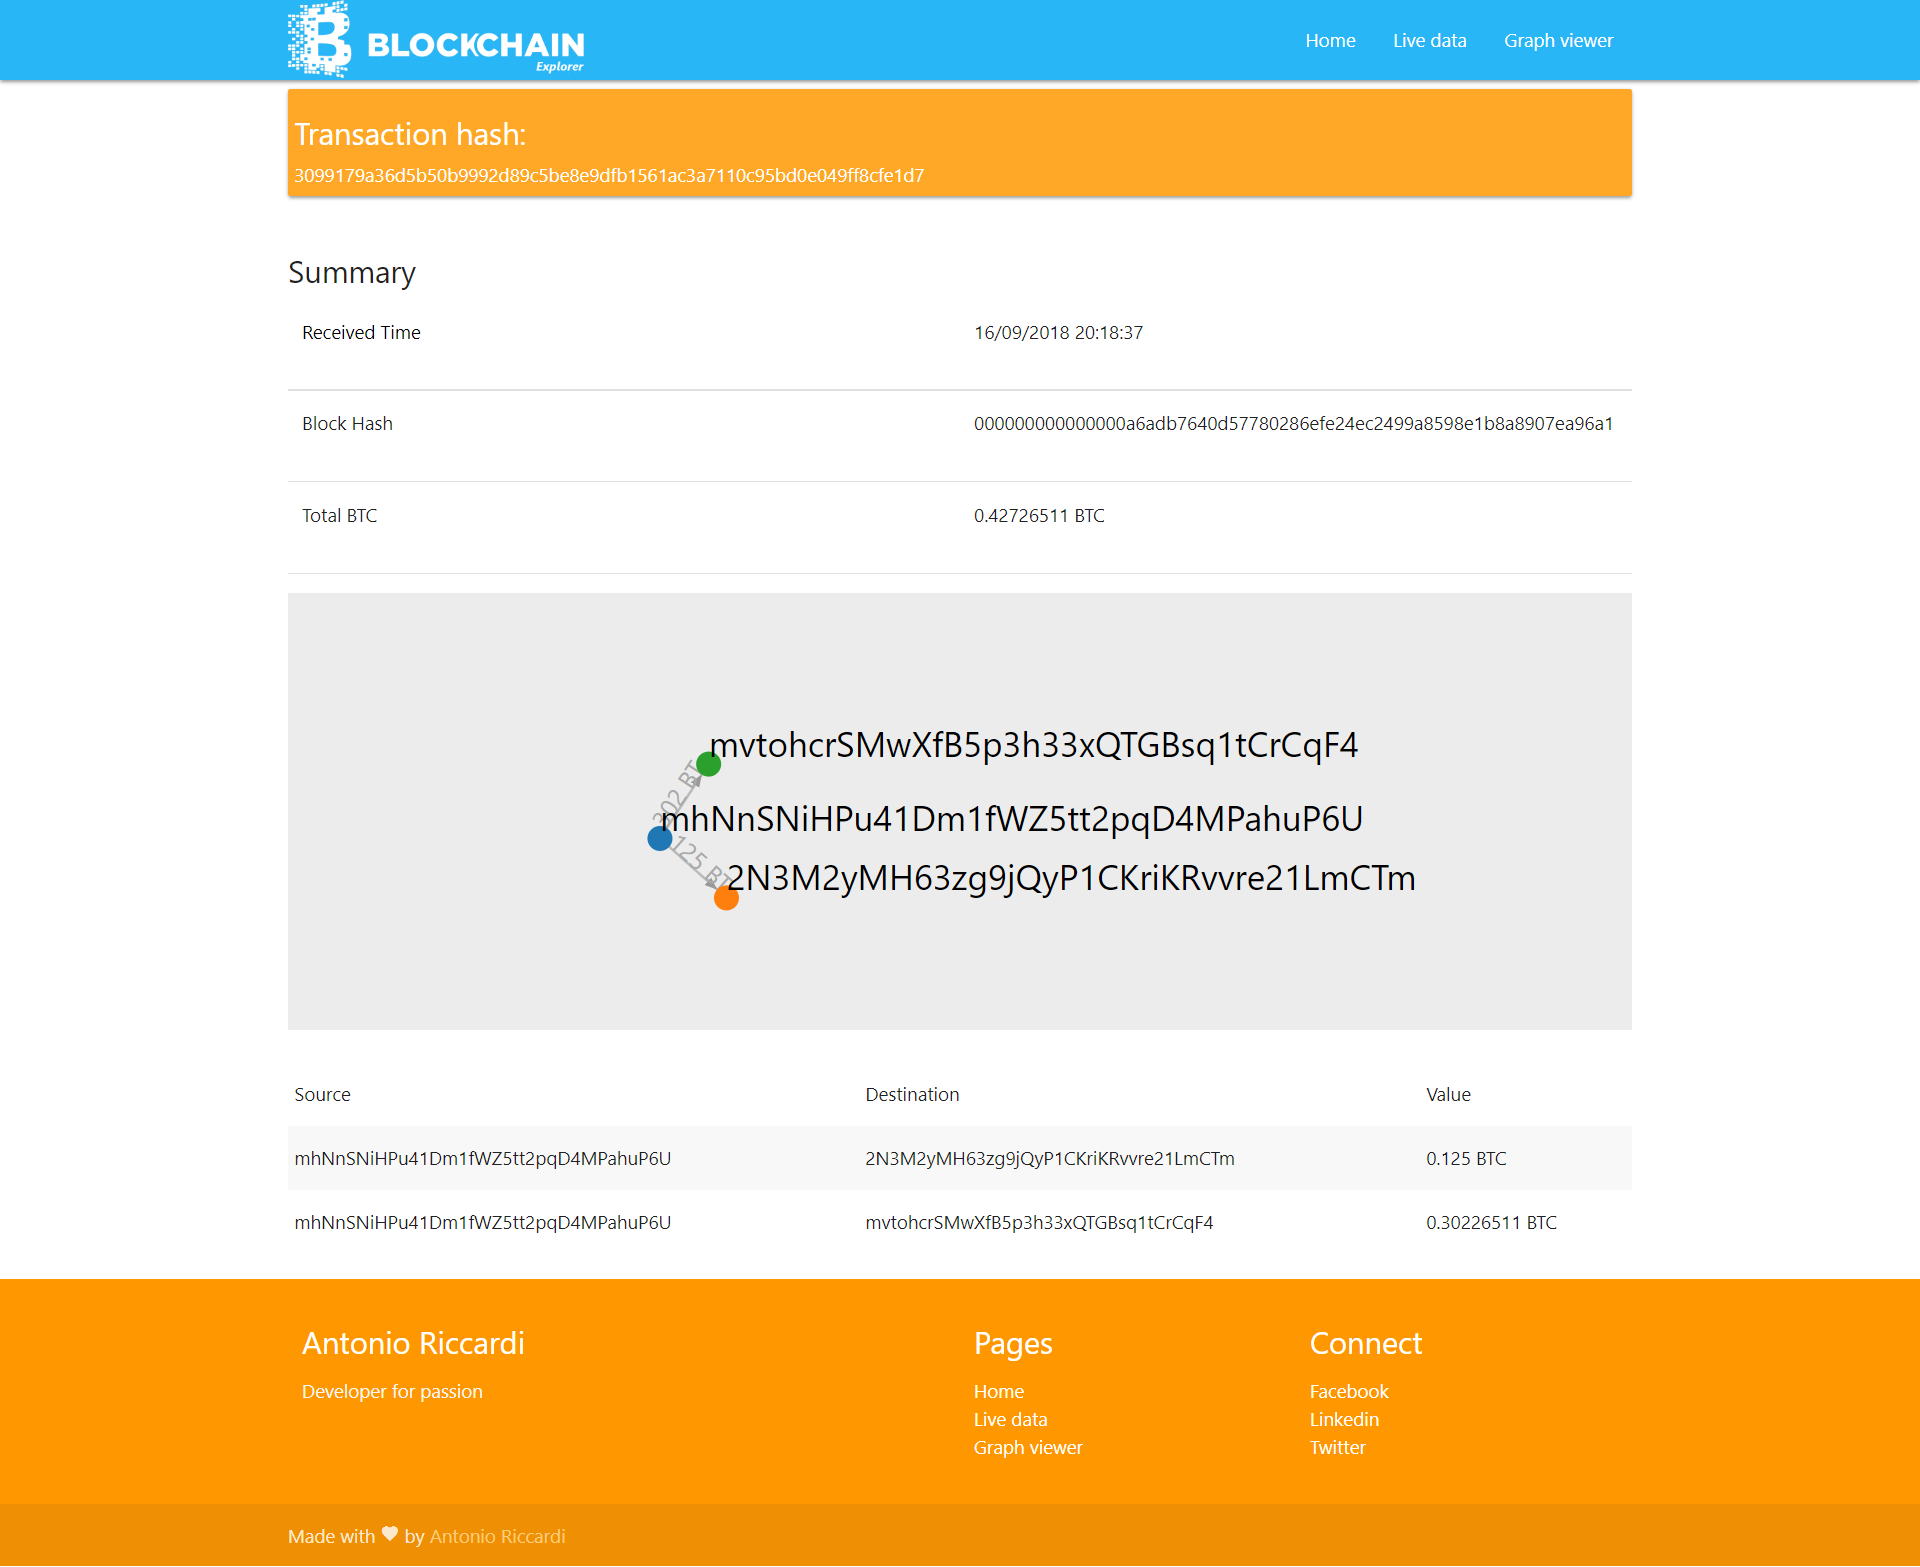
\includegraphics[width=\textwidth]{images/infoTransaction2.png}
	\caption{Dettaglio transazione.}
	\label{fig:transactionDetail}
\end{figure}
 
\item \textbf{Prelievo dati da Kafka}: Come detto in precedenza, il sistema distribuito al termine della propria elaborazione, pubblica i dati sui topic di Kafka. Blockchain Explorer, preleva i dati messi a disposizione dal topic di Kafka implementando un \textit{HighLevelConsumer}. L'oggetto in questione infatti si connette a Kafka e preleva i dati dal topic \textit{transaction-topic}. Infine li invia tramite websocket ai client che sono in ascolto sul server.
\begin{lstlisting}[language=Javascript, label=lst:kafka, caption={Creazione subscriber Kafka.}]

const kafkaBroker = config.kafka.host + ":" + config.kafka.port;
const client = new kafka.Client(kafkaBroker);
const topics = [
    {
        topic: config.kafka.topic
    }
];
const options = {
    autoCommit: true,
    encoding: 'utf8',
    groupId: 'bitcoin-webapp' //Math.random().toString()
};

const consumer = new kafka.HighLevelConsumer(client, topics, options);

consumer.on('message', function(message){
    console.log('Incoming message: ' + message.value.toString());
    wss.sendBrodcast(message.value.toString());
});
\end{lstlisting}

Il codice \ref{lst:kafka} mostra come la WebApp crea un HighLevelConsumer. Nello specifico viene creato un client, \textit{kafka.Client}, contenente l'IP e la porta di Kafka. Inoltre viene creato un oggetto \textit{topic} nella quale viene specificato il topic alla quale connettersi. I due oggetti, insieme ad altre opzioni \textit{options}, sono passate al costruttore dell'oggetto HighLevelConsumer il quale instaura una connessione con la coda e preleva i dati.
\\Infine, all'oggetto \textit{consumer} viene associata una funzione da eseguire ogni qualvolta un nuovo dato è disponibile. Questa funzione ha il compito di inviare i dati, tramite WebSocket, a tutti i client connessi al server.

\item \textbf{Comunicazione tramite Websocket}: Per permettere la comunicazione real-time delle transazioni provenienti da Kafka ai vari client, la WebApp crea un  server WebSocket. La creazione del server è visibile nel listato \ref{lst:websocket}.

\begin{lstlisting}[language=Javascript, label=lst:websocket, caption={Creazione di un Server WebSocket.}]
var wss = new webSocket.Server({
    port: config.webSocket.port
});


wss.sendBrodcast = function(message){
  wss.clients.forEach( function (client) {
     client.send(message);
  });
};
\end{lstlisting}

Infine, al Server WebSocket viene aggiunta la funzione \textit{sendBrodcast}, richiamata nel listato di Kafka \ref{lst:kafka}, la quale ha il compito di inviare a tutti i client connessi al server il messaggio, \textit{message}, proveniente da Kafka.
\item \textbf{Renderizzazione dei Grafi}: La renderizzazione dei grafi è demandata ai browser dei client. Il codice che segue viene inglobato nelle pagine HTML inviate dal server ai vari client. Il browser quindi, riceve dal server sia i dati che il codice da eseguire, generando una pagina come in figura \ref{fig:graphView}.

\begin{lstlisting}[language=Javascript, label=lst:intGraph, caption={Inizializzazione svg per il grafo.}]
var svg = d3.select("#" + idSvg),
        width = + $("#" + idSvg).width(),
        height = +svg.attr("height");

    var zoomLayer = svg.append('g');

    svg.call(d3.zoom().on('zoom', function(){
        zoomLayer.attr('transform', d3.event.transform);
    }));

    zoomLayer.append('defs').append('marker')
        .attrs({'id':'arrowhead',
            'viewBox':'-0 -5 10 10',
            'refX':13,
            'refY':0,
            'orient':'auto',
            'markerWidth':13,
            'markerHeight':13,
            'xoverflow':'visible'})
        .append('svg:path')
        .attr('d', 'M 0,-5 L 10 ,0 L 0,5')
        .attr('fill', '#999')
        .style('stroke','none');
\end{lstlisting}

Nel listato \ref{lst:intGraph} sono riportate le righe di codice che servono per l'inizializzazione del tag \textit{svg}, presente nella pagina HTML, nella quale verranno disegnate cerchi e le linee rappresentati rispettivamente nodi ed archi del grafo delle transazioni di bitcoin. Inoltre, su di esso viene aggiunto un layer per lo zoom, che permette all'utente finale di avere una fluida navigazione all'interno del grafo.

\begin{figure}[H]
	\centering
	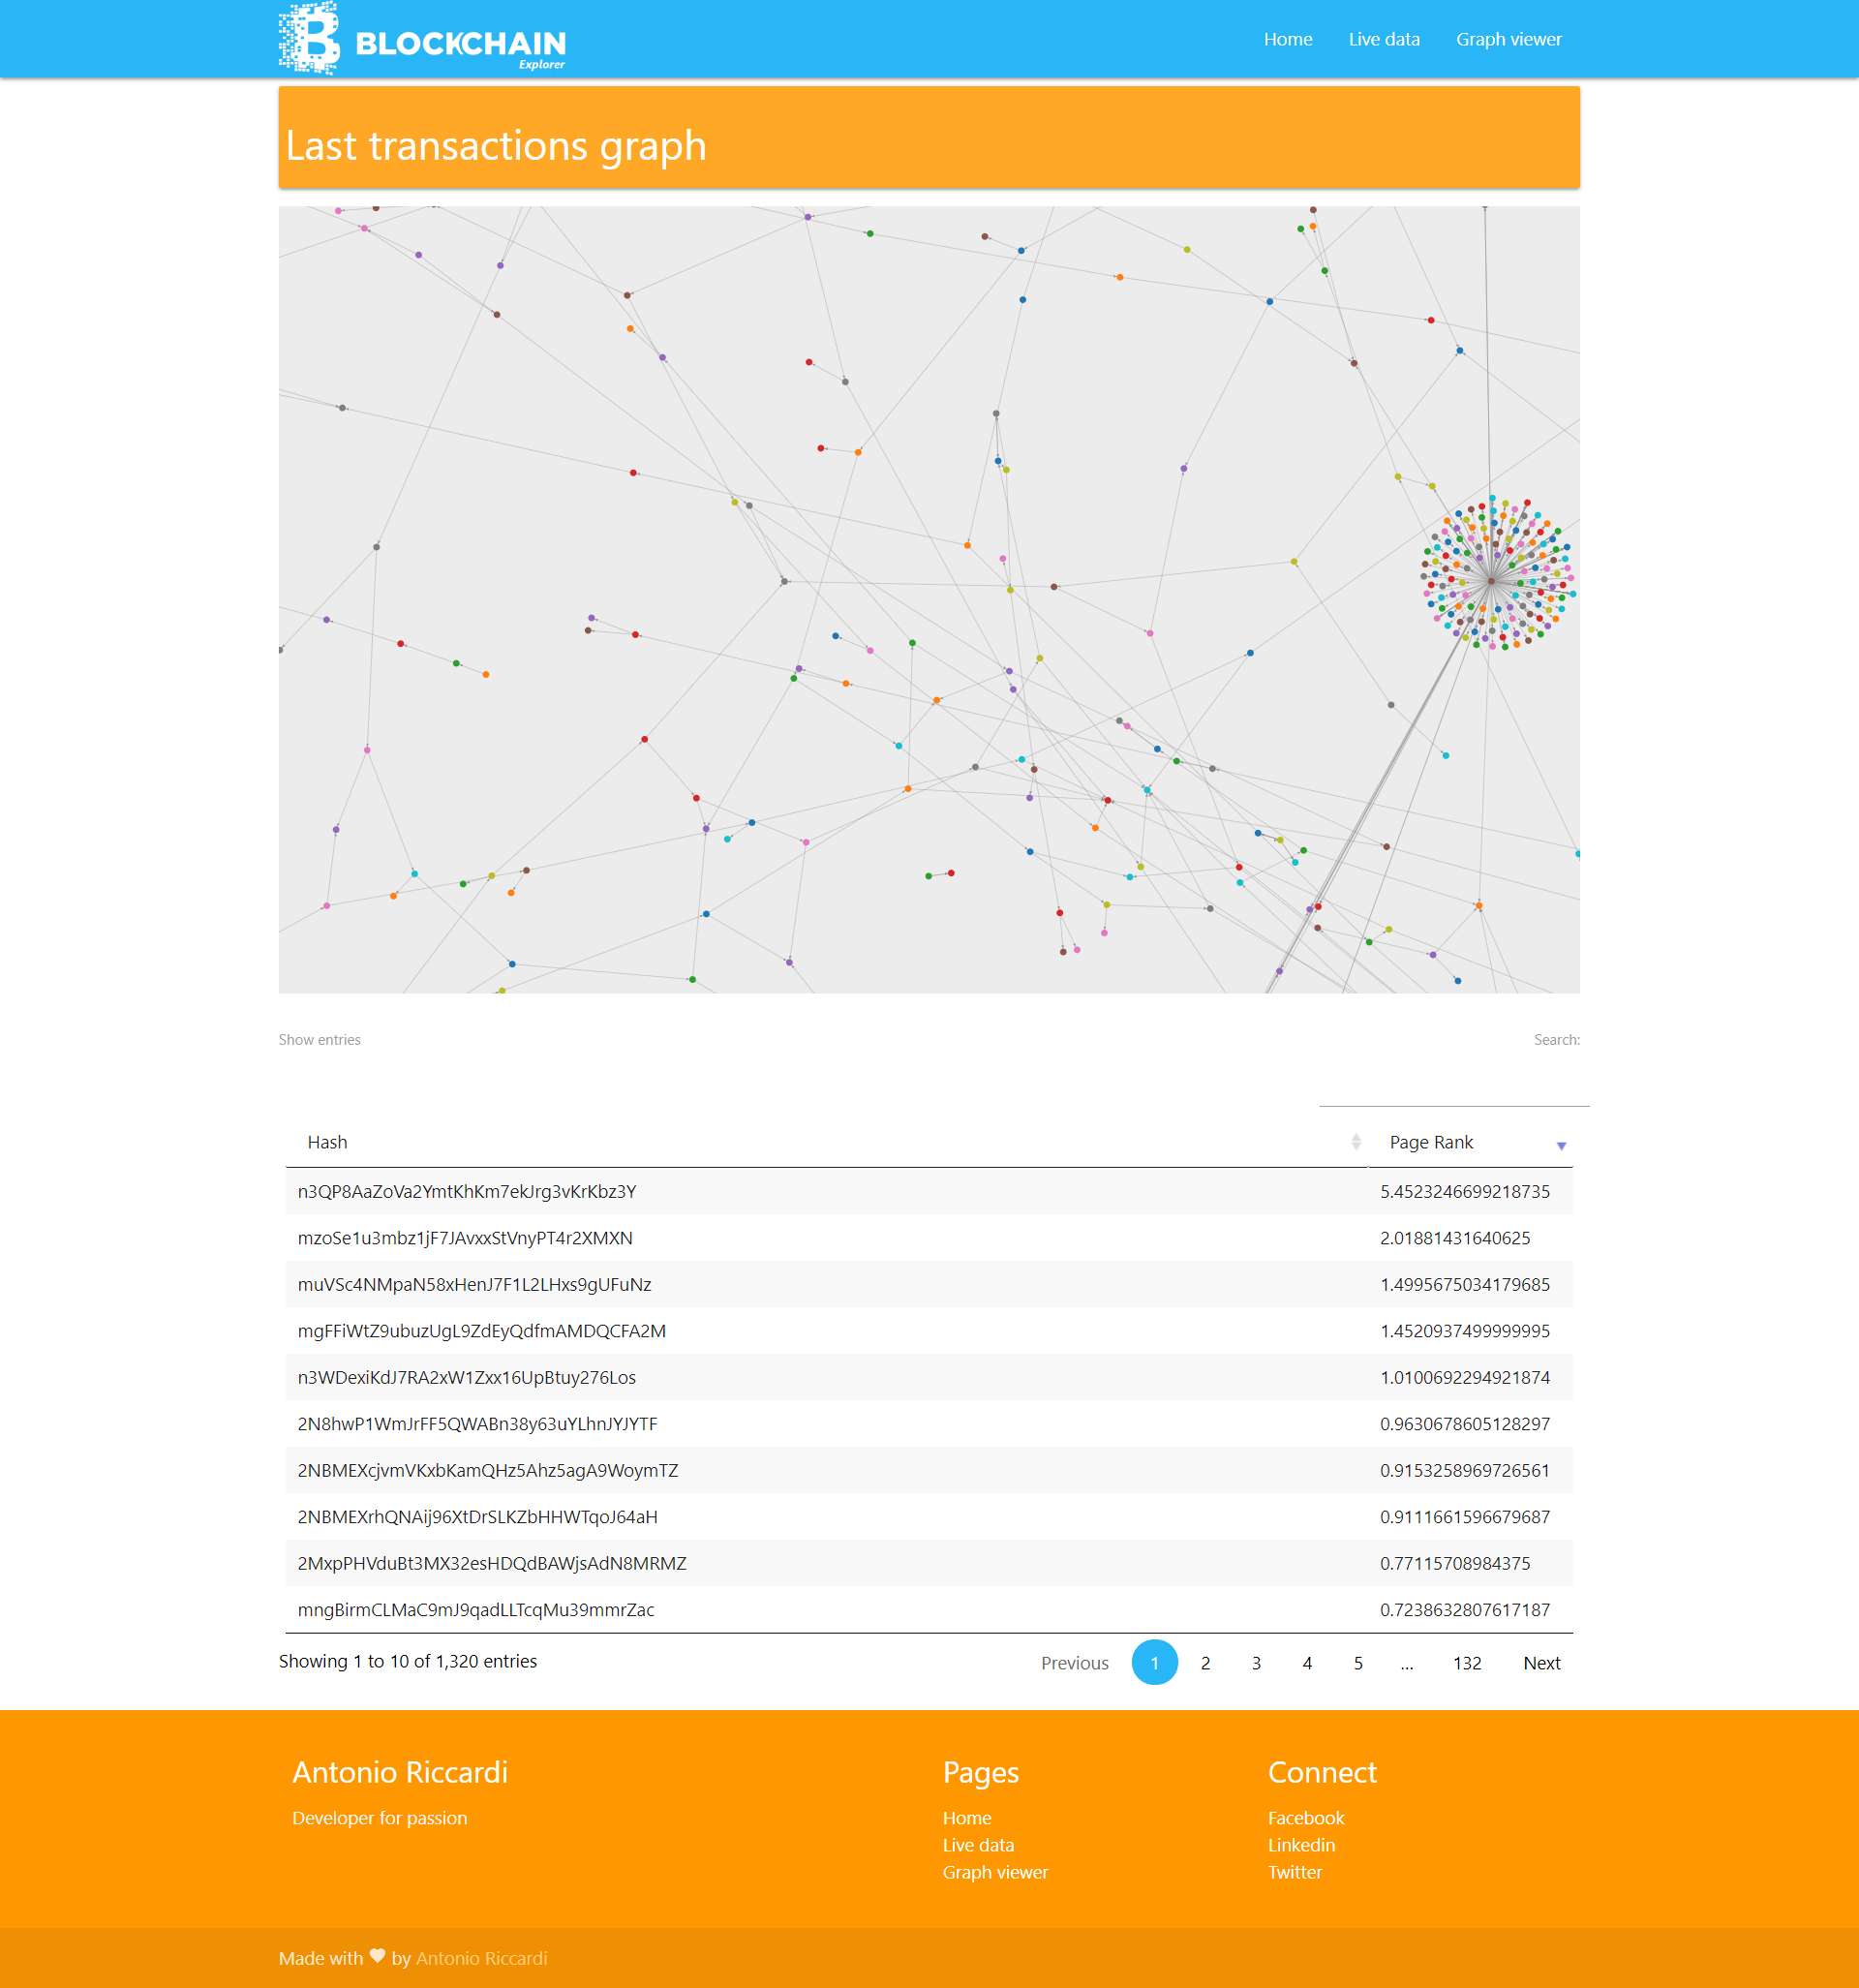
\includegraphics[width=\textwidth, height=0.50\textheight]{images/graphView.png}
	\caption{Grafo delle transazioni completo.}
	\label{fig:graphView}
\end{figure}


\begin{lstlisting}[language=Javascript, escapechar=|, label=lst:drawLine, caption={Creazione linee.}]
		simulation = d3.forceSimulation(nodes)
                            .force("link", d3.forceLink()
                            .id(function (d) { return d.hash;}))
                            .force("charge", d3.forceManyBody().strength(-80))
                            .force("center", d3.forceCenter(width / 2, height / 2))
                            .on("tick", tick)
                            .stop();

        simulation.force("link")|\label{line:link}|
            .links(links);

        for(i=0; i < 300; i++) simulation.tick();


        link.append("title")
            .text(function (d) {
                var t = "Transaction Hash: " + d.transactionHash + "\n" +
                        "Received Time: " + d.receivedTime + "\n" +
                        "Block Hash: " + d.blockHash + "\n" +
                        "Value: " + d.value;
                return t;

            });
\end{lstlisting}


Mentre, nel listato \ref{lst:drawLine} sono riportate le righe di codice utili alla creazione degli archi tra i vari nodi del grafo. In particolare, alla riga \ref{line:link} viene utilizzato il metodo \textit{link} di d3.js che prende in input i dati da renderizzare, i quali sono trasformati in elementi grafici dell'svg chiamati \textit{line}. A questi sono aggiunti le coordinate di partenza e destinazione, l'icona a forma di freccia e l'attributo \textit{title} contenente tutte le informazioni relative alla transazione (Hash, Timestam, valore totale della transazione e l'hash del blocco di appartenenza ).

\begin{lstlisting}[language=Javascript, escapechar=|, label=lst:drawNode, caption={Creazione dei nodi del grafo.}]

        node = zoomLayer
            .selectAll(".node")
            .data(nodes) |\label{line:nodes}|
            .enter()
            .append("g")
            .attr("class", "node")
            .attr("transform", function(d){ 
            return "translate(" + d.x + ", " + d.y + ")";})
            .on("contextmenu", function(data,index){
                console.info("Selected hash: " + data.hash);
                $("input[type='search']").val(data.hash);
                $("input[type='search']").keyup();
                d3.event.preventDefault();

            })
            .call(d3.drag()
                .on("start", dragstarted)
                .on("drag", dragged)
                .on("end", dragended)
            );

        node.append("circle")
            .attr("r", 5)
            .style("fill", function (d, i) {return colors(i);})


        node.append("title")
            .text(function (d) {return d.hash;});
\end{lstlisting}

Analogamente a quanto fatto per gli archi del grafo, nel listato \ref{lst:drawNode} viene mostrato come con D3.js sia possibile associare i dati esistenti in memoria ad elementi grafici sullo schermo. In questo caso, viene utilizzato il metodo \textit{data}, riga \ref{line:nodes}, per passare i nodi da disegnare nella pagina HTML al framework. I nodi, quindi, vengono disegnati tramite il tag \textit{circle} e correlati dalla classe \textit{node} che darà un colore diverso per ogni nodo. Infine, come accade agli archi, viene aggiunto un \textit{title} il quale contiene l'hash dei destinatari o mittenti delle transazioni.
 
\item \textbf{Costruzione delle tabelle}: Altro aspetto importante è la creazione delle tabelle. In Blockchain explorer è possibile visionare in forma tabellare le ultime transazioni processate, la sintesi di una transazione singola oppure i valori del PageRank per ogni hash. Nel codice \ref{lst:table}  è possibile vedere come sia facile trasformare una semplice \textit{<table>} HTML in una tabella con colonne ordinabili, paginazione e filtri di ricerca. Il tutto viene fatto dalla funzione \textit{DataTable(dataTableConfig)} il quale invoca la libreria DataTable che trasforma la tabella \textit{realTimeTransactions} con le proprietà inserite nella variabile \textit{dataTableConfig}.

\begin{lstlisting}[language=Javascript, label=lst:table, caption={Utilizzo DataTable.}]
var initializeTable = function(){
    transactionsTable = $('#realTimeTransactions').DataTable(dataTableConfig);
}

var dataTableConfig = {
    retrieve: true,
    data: [],
    dom: 'ftrip',
    order: [[2, 'desc']],
    columns:[
        {title: 'Transaction hash', className: '', orderable: false, visible: true},
        {title: 'Value Out', className: '', orderable: false, visible: true},
        {title: '', className: '', orderable: true, visible: false},
        {title: '', className: '', orderable: false, visible: false}
    ],
    oLanguage: {
        sEmptyTable: 'Waiting for transactions...'
    }
};
\end{lstlisting}

\item \textbf{HTML Templating}: Come detto in precedenza il server invia pagine HTML dinamiche partendo da template statici. Questa funzionalità è espletata da Express.js. In particolare la libreria permette di utilizzare un motore grafico per renderizzare le pagine HTML. Nell'elaborato di tesi viene utilizzato Handlebars. Il codice \ref{lst:render} mostra come sia semplice associare questo tool come motore grafico di Express. L'associazione viene fatta tramite il metodo \textit{engine}, il quale prende in ingresso una serie di informazioni quali: il template di default, le cartelle contenenti i template ed i partials ed una lista di funzioni, chiamate \textit{helpers}, che possono essere richiamate all'interno dell'HTML. 

\begin{lstlisting}[language=Javascript, label=lst:render, caption={Associazione Express-Handelbars.}]
// Create `ExpressHandlebars` instance with a default layout.
var hbs = exphbs.create({
    defaultLayout: 'main',
    layoutsDir: 'src/views/layouts/',
    partialsDir: 'src/views/partials/',
    helpers: {
        json : function(content) {
            return JSON.stringify(content);
        }
    }
});
app.engine('handlebars', hbs.engine);
\end{lstlisting}

Un template quindi non è altro che una pagina statica HTML, la quale in fase di run-time viene processata e modificata in base alle informazioni provenienti dal server. Un esempio di template è il listato \ref{lst:handleb}, il quale mostra la creazione dinamica delle righe della tabella, partendo dall'oggetto \textit{transaction} ricevuto dal server. Come si può notare, viene usato il costrutto \textit{each} per iterare sull'intero oggetto transaction e di prelevare solo le proprietà da inserire all'interno dei vari \textit{<td>}.

\begin{lstlisting}[language=Javascript, label=lst:handleb, caption={Template Handlebars.}]
<div class="row">
    <table class="table striped">

        <thead>
            <tr>
                <td>Source</td>
                <td>Destination</td>
                <td>Value</td>
            </tr>
        </thead>
        <tbody>
            {{#each transaction}}
                <tr>
                    <td>{{source.properties.hash}}</td>
                    <td>{{destination.properties.hash}}</td>
                    <td>{{relation.properties.value}} BTC</td>
                </tr>
            {{/each}}
        </tbody>
    </table>
</div>
\end{lstlisting}

%TODO Metti figura lista di transazioni

\begin{figure}[H]
	\centering
	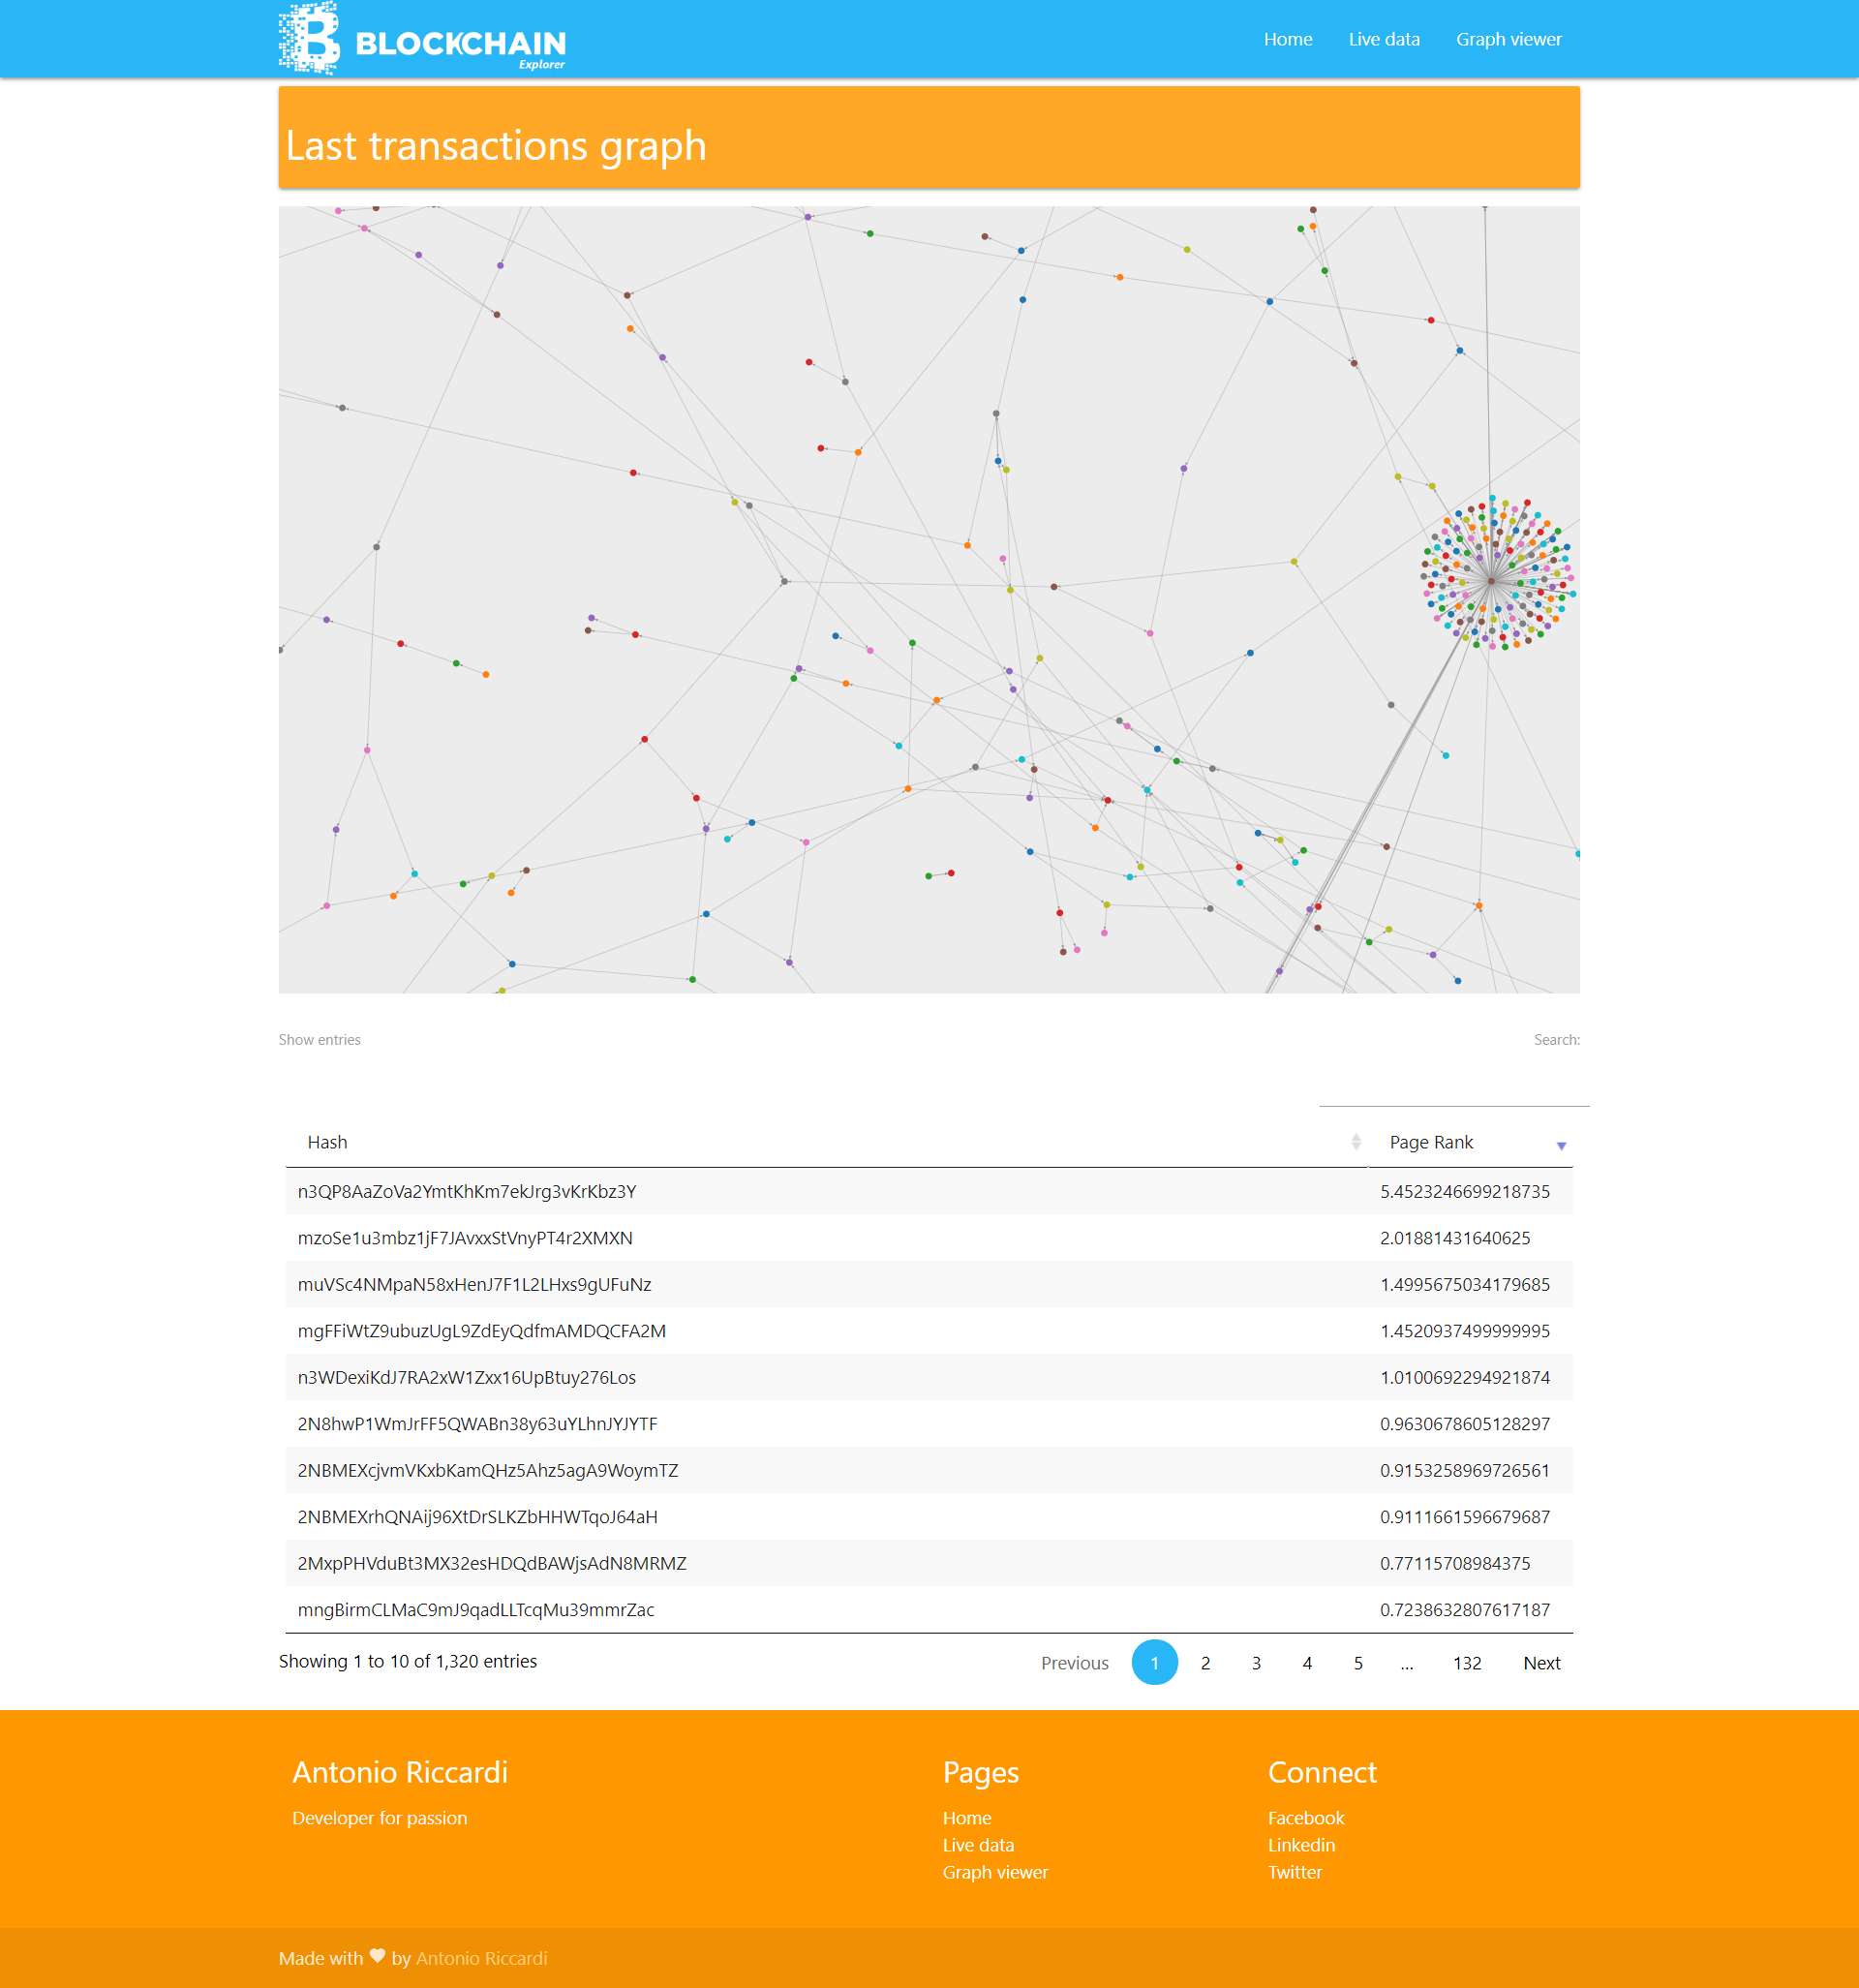
\includegraphics[width=\textwidth, height=0.80\textheight]{images/graphView.png}
	\caption{Grafo delle transazioni completo.}
	\label{fig:tableView}
\end{figure}

In figura \ref{fig:tableView} è possibile visualizzare la pagina HTML che viene generata dall'elaborazione del codice \ref{lst:handleb}. 

\end{itemize}
\section{GitHub}
\label{sec:github}
GitHub è un servizio di hosting per progetti software. Il nome "GitHub" deriva dal fatto che GitHub è una implementazione dello strumento di controllo versione distribuito \textit{Git} \cite{git:wiki}, inventato da Linus Torvalds anima e per anni programmatore di Linux. 
\\ GIT quindi è un version control system (VCS), e cioè un programma che permette di tener traccia di tutte le modifiche e le evoluzione effettuate nel corso della stesura di un codice o di un qualsiasi progetto su supporto digitale.
\\ Un software VCS permette di mantenere una copia del proprio codice
sorgente, sia in locale sia in remoto, senza incorrere in un eccessivo dispendio di energie e senza deconcentrarsi eccessivamente dalla stesure del proprio testo. In linea di principio un VCS permette di tenere sotto controllo qualsiasi documento, siano essi foto, documenti realizzati con programma di videoscrittura, fogli di calcolo, ecc.
\\ Git è diverso dai sistemi di controllo delle versioni precedenti come \textit{Subversion} in quanto è distribuito piuttosto che centralizzato. La differenza maggiore tra i due sistemi è la posizione del codice (repository): 
\begin{itemize}
\item \textbf{Centralizzato}: Tutto il software viene inviato dai programmatori direttamente ad un server centrale che detiene il repository.
\item \textbf{Distribuito}: Non esiste un server centrale, ma esistono repository locali (la macchina di sviluppo) e repository remoti (GitHub).
\end{itemize}
Per questo motivo, GIT è abbastanza veloce, soprattutto dal momento che la maggior parte delle operazioni avviene sul repository locale. Tuttavia, l'utilizzo di Git aggiunge un livello di complessità. L'invio di codice al repository locale e l'invio di commit a un repository remoto sono passaggi separati.
\\ GitHub dunque viene usato come repository remoto di Git da migliaia di sviluppatori poiché gratuito. Inoltre fornisce strumenti utili come il \textit{bug traking}, tool per controllare le differenze tra i file, possibilità di visualizzare cronologia dei commit ed una sezione per commenti ed suggerimenti.
\\ Per l'elaborato di tesi è stato usato questo sistema per tenere traccia delle modifiche apportate al codice. Questo ha permesso in molti casi di ripristinare una versione funzionante del software dopo l'immissione di nuove modifiche. GitHub inoltre, è stato utilizzato per permettere a chiunque volesse riprendere il progetto, modificarlo o applicare delle correzioni, semplicemente \textit{clonando} il repository.
\\I due elaborati di tesi possono essere clonati ai seguenti URL:
\begin{itemize}
\item \textbf{Sistema Distribuito}: \href{https://github.com/Antonio90/BitcoinSpark.git}{https://github.com/Antonio90/BitcoinSpark.git}.
\item \textbf{Blockchain Explorer}: \href{https://github.com/Antonio90/bitcoin-webapp.git}{https://github.com/Antonio90/bitcoin-webapp.git}. 
\end{itemize}
\chapter{Conclusioni e sviluppi futuri}
\label{chap:conclusioni e sviluppi futuri}
\Blindtext

%\appendix
% INCLUSIONE APPENDICI - - PERSONALIZZARE - TENERE COERENTE CON LISTA IN ALTO
%\chapter{An appendix}
\label{app:a}
\Blindtext



% BIBLIOGRAFIA

\nocite{*}
\printbibliography
\addcontentsline{toc}{chapter}{\refname}

\end{document}